
\documentclass[a4paper, 12pt]{report}

% Adapté du tempate TER-M1 de l'Université de Paris

%%%%%%%%%%%%
% Packages %
%%%%%%%%%%%%

\usepackage{lipsum}
\usepackage[french]{babel}
%\usepackage{hyperref}
\usepackage[noheader]{packages/sleek}
\usepackage{packages/sleek-title}
\usepackage[french]{packages/sleek-theorems}
\usepackage{packages/sleek-listings}
\usepackage{tikz}
\usepackage[french,linesnumbered,lined]{algorithm2e}
\SetKwInput{KwResult}{R\'esultat}
\SetKw{KwInput}{Entr\'ees}
%%%%%%%%%%%%%%
% Title-page %
%%%%%%%%%%%%%%

\logo{./resources/img/logo_science.png}
\institute{Sorbonne Université}
\faculty{Master ANDROIDE / AI2D}
\title{Institut des Systèmes Intelligents et de Robotique (ISIR)}
\subtitle{Stage de Master 1}
\author{ Réalisé par : \\[0.5cm]
		\textbf{Paul \textsc{Chambaz}    }       \\[1cm]
		Encadré par :        \\
		M. Olivier Sigaud, ISIR, Sorbonne Université \\[1cm]
		Référent  :        \\
		M. Thibaut Lust, LIP6, Sorbonne Université
		 }

%%%%%%%%%%%%%%%%https://www.overleaf.com/project/6012bd305aee4065605e8f1d
% Bibliography %
%%%%%%%%%%%%%%%%

\addbibresource{references.bib}

%%%%%%%%%%
% Others %
%%%%%%%%%%

\lstdefinestyle{latex}{
    language=TeX,
    style=default,
    %%%%%
    commentstyle=\ForestGreen,
    keywordstyle=\TrueBlue,
    stringstyle=\VeronicaPurple,
    emphstyle=\TrueBlue,
    %%%%%
    emph={LaTeX, usepackage, textit, textbf, textsc}
}

\FrameTBStyle{latex}

\def\tbs{\textbackslash}

%%%%%%%%%%%%
% Document %
%%%%%%%%%%%%

\begin{document}
    \maketitle
    \romantableofcontents

    \chapter{Introduction}

    L'apprentissage par renforcement permet à un agent d'apprendre à prendre
    des décisions optimales dans un environnement en interagissant avec
    celui-ci. Dans les applications modernes, ces agents utilisent des réseaux
    de neurones pour estimer la valeur des actions possibles, mais ces
    estimations comportent des erreurs. Ces erreurs, appelées biais
    d'estimation, peuvent se propager et s'amplifier durant l'apprentissage,
    ce qui dégrade la qualité des choix d'actions.

    Un problème particulier survient quand l'agent doit choisir l'action de
    plus forte valeur estimée : il sélectionne les actions
    surestimées par le bruit, créant un cycle qui amplifie les erreurs. Pour
    contrer ce « biais de maximisation », des méthodes « pessimistes »
    sous-estiment délibérément les valeurs. Des algorithmes récents (TQC, TOP,
    BAC) proposent des mécanismes sophistiqués pour contrôler ce pessimisme,
    mais certains résultats récents remettent en cause leur efficacité.

    Ce stage à l'ISIR a porté sur l'étude empirique de ces mécanismes. Une
    infrastructure logicielle a été développée pour comparer plusieurs
    algorithmes et une méthodologie de mesure du biais par simulation Monte
    Carlo a été mise en place. Le travail s'est articulé autour de plusieurs
    axes : la reproduction d'expériences de la littérature, l'étude comparative
    sur l'environnement MountainCar Continuous et l'investigation de
    l'algorithme AFU.

    Cette démarche a révélé des comportements inattendus : une erreur
    méthodologique dans une figure d'un article qui invalidait ses
    conclusions, des mécanismes de gestion du biais différents
    dans AFU et l'absence de corrélation claire entre contrôle du biais et
    performance d'apprentissage sur l'environement MountainCar Continuous.

    \chapter{Contexte}

    \section{Modélisation}

  L'apprentissage par renforcement modélise la prise de décision séquentielle à
  travers les Processus de Décision Markoviens (MDP) \cite{10.5555/3312046}. Un
  MDP est défini par le quintuplet $(\cal{S}, \cal{A}, \cal{P}, \cal{R},
  \gamma)$ où :


    \begin{itemize}
      \item $\cal{S}$ représente l'espace des états possibles de l'environnement ;
      \item $\cal{A}$ représente l'espace des actions disponibles à l'agent ;
      \item $\cal{P} : \cal{S} \times \cal{A} \times \cal{S} \rightarrow [\text{0}, \text{1}]$ définit les probabilités de transitions entre états ;
      \item $\cal{R} : \cal{S} \times \cal{A} \rightarrow \mathbb{R}$ attribue une récompense à chaque couple état-action ;
      \item $0 \leq \gamma < 1$ est le facteur d'actualisation qui pondère les récompenses futures.
    \end{itemize}

    Une politique $\pi : \cal{S} \times \cal{A} \rightarrow [\text{0},
    \text{1}]$ détermine le comportement de l'agent en spécifiant $\pi(a|s)$,
    la probabilité de choisir l'action $a$ dans l'état $s$. Pour les politiques
    déterministes, on note simplement $\pi : \cal{S} \rightarrow \cal{A}$ où
    $\pi(s)$ donne l'action choisie dans l'état $s$.

    Le retour cumulé actualisé à partir du pas de temps $t$ sous la politique
    $\pi$ s'exprime comme :

    $$
    G_t^\pi = \sum_{k=0}^\infty \gamma^k R_{t+k+1},
    $$

    où $R_{t+k+1} = {\cal{R}}(S_{t + k}, A_{t + k})$ représente la récompense reçue à l'instant $t+k+1$.
  
    \section{TD Learning}

    Les fonctions valeur quantifient la qualité des états et des actions . La
    fonction valeur d'état $V^\pi (s)$ et la fonction valeur d'action $Q^\pi
    (s, a)$ sous la politique $\pi$ sont définies par :

    $$
    V^\pi (s) = \mathbb{E}_\pi [ G_t | S_t = s],
    $$

    $$
    Q^\pi (s, a) = \mathbb{E}_\pi [ G_t | S_t = s, A_t = a].
    $$

    La politique optimale $\pi^*$ maximise les retours espérés depuis tous les états, avec les fonctions valeur optimales correspondantes $V^* (s) = \max_\pi V^\pi (s)$ et $Q^* (s, a) = \max_\pi Q^\pi (s, a)$. Ces fonctions satisfont les équations d'optimalité de Bellman :

    $$
    V^* (s) = \max_a \mathbb{E} [R_{t+1} + \gamma V^* (S_{t+1}) | S_t = s, A_t = a],
    $$

    $$
    Q^* (s, a) = \mathbb{E} [R_{t+1} + \gamma \max_{a'} Q^* (S_{t+1}, a') | S_t = s, A_t = a].
    $$

    L'apprentissage par différence temporelle (TD) approxime ces fonctions
    valeur par des mises à jour itératives. La règle de
    mise à jour Q-learning pour apprendre $Q^*$ est :

    $$
    Q(S_t, A_t) \leftarrow Q(S_t, A_t) + \alpha [R_{t+1} + \gamma \max_a Q(S_{t+1}, a) - Q(S_t, A_t)],
    $$

    où $\alpha$ est le taux d'apprentissage. Cette mise à jour utilise le
    bootstrapping : l'estimation courante sert à former la cible pour la mise à
    jour.

    \section{Méthode de Policy Gradient}

    Dans l'apprentissage par renforcement profond, la fonction $Q$ est
    approximée par un réseau de neurones $Q_\theta (s, a)$ avec des paramètres
    $\theta$ \cite{sutton1999policygradientmethodsreinforcement}. Le réseau est
    entraîné en minimisant l'erreur de différence temporelle, qui compare
    l'estimation courante avec la cible $y$ :

    $$
    y = r + \gamma \max_{a'} Q_\theta (s', a'),
    $$

    $$
    {\cal{L}}_Q (\theta) = \mathbb{E}_{(s,a,r,s') \sim \cal{B}} [(Q_\theta (s, a) - y)^2 ].
    $$

    Pour le contrôle continu, calculer $\max_{a'} Q_\theta (s', a')$ sur des
    espaces d'actions continus est impossible. Les méthodes acteur-critique
    résolvent ce problème en maintenant un réseau de politique séparé $\pi_\phi
    (s)$ qui produit directement les actions. La cible devient alors :

    $$
    y = r + \gamma Q_\theta (s', \pi_\phi (s')).
    $$

    L'utilisation de bootstrap dans l'apprentissage TD crée des instabilités
    potentielles, en particulier quand la cible dépend des paramètres $\theta$
    qui sont simultanément mis à jour. Les réseaux cibles résolvent ce problème
    en maintenant des copies lentement mises à jour $\theta^-$ pour le calcul
    des cibles, où $\theta^- \leftarrow \tau \theta + (1 - \tau) \theta^-$.

    $$
    {\cal{L}}_Q (\theta) = \mathbb{E}_{(s,a,r,s') \sim \cal{B}} [(Q_\theta (s, a) - r - \gamma Q_{\theta^-} (s', \pi_\phi (s')))^2 ].
    $$

    Les transitions $(s, a, s', r)$ représentent alors les exemples et les
    cibles sont alors les étiquettes à apprendre par le réseau. Pour que les
    exemples ne soient pas trop corrélés entre eux, chaque transition est
    placée dans un replay buffer $\cal{B}$. Lors de l'apprentissage, un
    mini-batch est échantillonné uniformément parmi ce replay buffer.

    \section{Biais d'estimation}

    Dans l'apprentissage par renforcement profond, l'approximation des
    fonctions valeur par des réseaux de neurones introduit inévitablement des
    erreurs d'estimation \cite{thrun1993issuesactionselection}. Ces erreurs,
    lorsqu'elles sont amplifiées par le processus de bootstrap, peuvent
    compromettre significativement l'efficacité de l'apprentissage. Le biais
    d'estimation représente l'écart systématique entre la fonction valeur
    associée à la politique courante $\pi$ et son estimation par le réseau de
    neurones. On note :

    $$
    \text{Bias} = \mathbb{E} [ Q_\theta (s, a) - Q^\pi (s, a)].
    $$

    Ce biais peut être positif ou négatif, on parle alors de surestimation et
    de sous-estimation respectivement. Un biais peut devenir problématique dans
    le contexte de l'apprentissage par renforcement car il se propage et
    s'amplifie à travers les équations de Bellman.

    \subsection{Biais de maximisation}

    Le biais de maximisation constitue l'une des principales sources
    d'instabilité dans l'apprentissage par renforcement. Il émane directement
    de la structure de l'équation de différence temporelle qui utilise
    l'opérateur maximum :

    $$
    y = r + \gamma \max_{a'} Q_\theta (s', a').
    $$

    Lorsque $Q_\theta (s, a)$ contient du bruit d'estimation, l'opérateur max
    sélectionne préférentiellement les erreurs positives. Considérons une
    décomposition de notre estimation bruitée :

    $$
    Q_\theta (s, a) = Q^\pi (s, a) + \epsilon (s, a),
    $$

    où $\epsilon (s, a)$ représente l'erreur d'estimation de moyenne nulle.
    L'inégalité de Jensen nous donne :

    $$
    \mathbb{E} [ \max_{a'} (Q^\pi (s', a') + \epsilon (s', a')) ] \geq \max_{a'} \mathbb{E} [ Q^\pi (s', a') + \epsilon (s', a')] = \max_{a'} Q^\pi (s', a').
    $$

    Cette inégalité montre que l'espérance du maximum des estimations bruitées
    dépasse systématiquement le maximum des valeurs. Plus le bruit d'estimation
    est important, plus cette surestimation s'amplifie.

    L'opérateur $\max$ cause le problème : il sélectionne la plus haute
    valeur, alors que cette valeur peut être la plus haute non pas car elle est
    effectivement associée à la meilleure action, mais plutôt à cause du
    bruit. Cette action sous-optimale génère ensuite des cibles biaisées qui se
    propagent dans tout le réseau via les mises à jour de Bellman, créant un
    cycle de surestimation.

    \subsection{Double TD Learning}

    Le double Q-learning \cite{hasselt2010doubleqlearning} tente de résoudre ce
    problème en découplant la sélection de l'action de son évaluation. L'idée
    consiste à maintenir deux estimateurs indépendants $Q_A$ et $Q_B$ et à
    utiliser l'un pour sélectionner l'action et l'autre pour l'évaluer :

    $$
    y = r + \gamma Q_B (s', \arg\max_{a'} Q_A (s', a')).
    $$

    Cette approche fonctionne bien dans les espaces d'actions discrets car les
    erreurs dans $Q_A$ et $Q_B$ sont supposées indépendantes. Cependant, dans
    les méthodes acteur-critique pour le contrôle continu, cette indépendance
    est compromise pour plusieurs raisons :

    \begin{itemize}
      \item les deux critiques sont entraînés sur le même mini-batch, créant des corrélations dans leurs erreurs ;
      \item les réseaux partagent souvent des architectures identiques, conduisant à des biais structurels similaires ;
      \item les deux critiques évaluent les actions de la même politique introduisant des dépendances supplémentaires.
    \end{itemize}

    \section{Méthodes pessimistes}

    Pour tenter de résoudre les limitations du double TD-learning classique, on
    utilise une approche différente basée sur le pessimisme.

    TD3 (Fujimoto et al. 2018) introduit le pessimisme systématique. Au moment
    du calcul des cibles, plutôt que d'utiliser l'estimateur $Q_\theta$, on
    crée un nouvel estimateur artificiel qui est une borne pessimiste
    $Q^\text{pes}_\theta$.

    Ce pessimisme a pour objectif de contrer la surestimation induite par le
    biais de maximisation. De plus, par la nature de l'opérateur $\arg\max_a$,
    ici remplacé par $\pi_\phi$ pour les actions continues, les erreurs de
    sous-estimation ne se propagent pas de la même façon que les erreurs de
    surestimation dans le processus de bootstrap. On peut donc être
    artificiellement pessimiste, ce qui permet dans l'idéal de résoudre le
    biais de maximisation. Si l'on est en fait trop pessimiste, la valeur
    ne se propage pas dans les états adjacents (mais peut impacter
    l'apprentissage de l'acteur). Ce cadre pessimiste ouvre la voie à des
    méthodes plus sophistiquées comme TD3, TQC ou TOP.

    \subsection{TD3}

    Twin Delayed Deep Deterministic Policy Gradient (TD3), qui a introduit la
    notion de pessimisme pour résoudre le biais de maximisation dans le cadre
    des actions continues
    \cite{fujimoto2018addressingfunctionapproximationerror}, propose une façon
    d'être pessimiste. Au lieu de prendre un réseau critique, on en utilise
    deux, $Q_{\theta_1}$ et $Q_{\theta_2}$, et on prend leur minimum lors du
    calcul des cibles :

    $$
    y = r + \gamma \min (Q_{\theta^-_1} (s', \pi_{\phi} (s')), Q_{\theta^-_2} (s', \pi_{\phi} (s'))).
    $$

    Cette approche crée une borne pessimiste : si les deux critiques
    surestiment indépendamment à cause du bruit, le minimum fournit une
    estimation plus conservatrice.

    \subsection{TQC}

    Truncated Quantiles Critics (TQC) adopte une approche distributionnelle en
    modélisant la distribution complète des retours plutôt qu'une simple
    espérance \cite{kuznetsov2020controllingoverestimationbiastruncated}.
    Chaque critique $Z_\psi (s, a)$ produit $M$ quantiles de la distribution
    des valeurs :

    $$
    Z_\psi (s, a) = { \theta^1_\psi (s, a), \theta^2_\psi (s, a), ..., \theta^M_\psi (s, a)}.
    $$

    L'entraînement utilise une régression quantile
    \cite{dabney2017distributionalreinforcementlearningquantile} :

    $$
    {\cal{L}}_Z (\psi) = \mathbb{E} [ \frac{1}{N M} \sum_{m=1}^M \sum_{i=1}^N \rho^\tau_H (y_i - \theta^m_\psi (s, a)) ],
    $$

    où ${\rho^\tau_H} = \mid {\tau} - \mathbb{I} (u < 0) \mid {\cal{L}}^1_H
    (u)$ est la perte quantile avec régularisation de Huber.

    Pour induire du pessimisme, TQC propose la troncature des quantiles. Après
    avoir collecté tous les quantiles de tous les critiques, on trie l'union et
    on supprime les $d \times N$ quantiles les plus élevés. La distribution
    obtenue sert alors de distribution cible à l'apprentissage des
    distributions des critiques. Cette troncature permet donc un niveau de
    contrôle plus précis via les paramètres $d$ et $M$.

    L'incertitude aléatoire signifie l'incertitude présente dans la
    connaissance du problème sous-jacent, mais qui ne peut pas être apprise et
    qui est directement liée à la stochasticité inhérente à l'environnement et
    à la modélisation. En modélisant les retours non pas sous la forme d'une
    espérance mais d'une distribution, TQC capture l'incertitude aléatoire et
    l'utilise comme moyen de générer du pessimisme.

    \subsection{TOP}

    Tactical Optimism and Pessimism (TOP) utilise un ensemble de critiques et
    combine l'espérance et la variance des estimations de cet ensemble pour
    gérer le niveau de pessimisme
    \cite{moskovitz2022tacticaloptimismpessimismdeep} :

    $$
    y = r + \gamma (\mathbb{E}_i [ Z_i(s', \pi(s')) ] + \beta \text{Var}_i [ Z_i(s' ,\pi(s')) ]).
    $$

    Le paramètre $\beta$ gère alors le niveau précis d'optimisme ou de
    pessimisme à utiliser. De plus, TOP propose l'utilisation d'un problème de
    bandit multi-bras opérant à l'échelle des épisodes. À chaque début
    d'épisode, un $\beta$ est sélectionné selon une distribution de probabilité
    $p_m (\beta)$ et cette distribution est mise à jour en fin d'épisode selon
    la performance. Cette approche permet d'adapter automatiquement le niveau
    d'optimisme ou de pessimisme en fonction des phases d'apprentissage.

    L'incertitude épistémique signifie l'incertitude directement liée au manque
    de connaissance du problème et est à distinguer de l'incertitude aléatoire.
    Le désaccord entre les critiques est fortement lié à l'incertitude
    épistémique, donc TOP l'utilise comme moyen de générer du pessimisme. Ce
    type d'incertitude est voué à disparaître sur un horizon infini. Cela veut
    dire que les méthodes qui l'utilisent, comme TOP ou TD3 (car le target de
    TD3 se ramène au target de TOP avec $N=2$ et $\beta = -\frac{\sqrt{2}}{2}$)
    génèrent de moins en moins de pessimisme au fur et à mesure que
    l'entraînement avance.

    \subsection{BAC}

    Blended Exploration Exploitation Actor-Critic (BAC) adopte une autre façon
    de gérer le niveau d'optimisme ou de pessimisme
    \cite{ji2024seizingserendipityexploitingvalue}. Tout d'abord, on note que
    l'on peut souffrir de pessimisme si le réseau courant $\pi$ a « oublié »
    les meilleures actions de certains états. Pour réduire cela, on peut
    apprendre sur les données historiques du replay buffer un estimateur
    $V_\psi(s)$ qui apprend pour chaque état la valeur du $\max_a Q(s', a)$
    avec une régression d'expectile de paramètre $\tau = 0,7$. On peut alors
    créer une nouvelle cible :

    $$
    y = r + \gamma (\lambda T^\pi_{\text{explore}} (s', a') + (1 - \lambda) T^\pi_{\text{exploit}} (s', a')),
    $$

    $$
    T^\pi_{\text{explore}} (s', a') = \mathbb{E}_{s',a'} [ Q(s', a') - \alpha log \pi(a'|s')],
    $$

    $$
    T^\pi_{\text{exploit}} (s', a') = \mathbb{E}_{s'} [V_\psi (s')].
    $$

    Cette cible contient deux sous-opérateurs, $T^\pi_{\text{explore}}$ et
    $T^\pi_{\text{exploit}}$, l'un correspondant à l'opérateur standard utilisé
    dans les frameworks de maximisation de l'entropie et qui encourage
    l'exploration et l'autre, mélangé avec le premier, qui apprend à
    sélectionner la valeur associée aux meilleures actions. Du fait que le
    paramètre de l'expectile regression est faible ($\tau = 0,7$), on peut
    aussi encourager du pessimisme par rapport à une simple cible.

    \chapter{Contributions}

    \section{Infrastructure}

    Avant de pouvoir contribuer à la recherche sur le biais d'estimation, il a
    fallu une période d'apprentissage pour étudier et comprendre les
    algorithmes utilisés. Si j'avais déjà travaillé avec TD3 , SAC
    \cite{haarnoja2019softactorcriticalgorithmsapplications} et AFU
    \cite{perringilbert2024afuactorfreecriticupdates} par le passé, certains
    aspects de ces algorithmes restaient incompris. Trois algorithmes récents
    nécessitaient une étude approfondie : TQC , TOP et BAC . Ces méthodes,
    publiées entre 2020 et 2024, représentaient des approches nouvelles pour
    gérer le biais d'estimation en apprentissage par renforcement continu.

    L'implémentation de ces algorithmes s'est révélée être un moyen efficace
    pour comprendre leurs mécanismes internes. Cette démarche pratique permet
    de saisir les détails techniques qui ne transparaissent pas toujours dans
    les descriptions théoriques des articles. Chaque implémentation révèle les
    choix d'architecture, les ordres de mise à jour des réseaux et les
    subtilités numériques qui influencent la performance des algorithmes.

    Le travail a commencé avec des implémentations en PyTorch, framework que
    j'utilisais habituellement. Cependant, les difficultés rencontrées pour
    gérer les fonctions de perte jointes d'AFU ont motivé une transition vers
    JAX. Cette migration technique s'est révélée bénéfique à plusieurs niveaux.
    JAX offre une approche fonctionnelle mieux adaptée aux algorithmes
    d'apprentissage par renforcement, où les mises à jour de paramètres et les
    calculs de gradients peuvent être exprimés de manière plus explicite. La
    performance obtenue avec JAX sur les applications étudiées s'est révélée
    environ cinq fois supérieure à celle de PyTorch, ce qui a accéléré les
    expériences.

  \begin{lstlisting}[language=Python]
  class RLAlgo:
      def __init__():
      def select_action(self, state, evaluation):
      def evaluate(self, state, action):
      def push_buffer(self, state, action, reward, next_state, done):
      def update(self):
      def get_state(self):
      def load_from_state(self, state):
  \end{lstlisting}

    L'ensemble des implémentations développées suit une interface commune
    appelée RLAlgo, qui définit les méthodes standards que tout algorithme
    d'apprentissage par renforcement doit implémenter : sélection d'action,
    mise à jour du replay buffer, pas d'entraînement et sauvegarde/chargement
    d'état. Cette interface uniforme facilite les comparaisons entre
    algorithmes et permet d'analyser leurs comportements dans des conditions
    identiques. Les algorithmes implémentés incluent SAC, TD3, TQC, TOP, AFU
    ainsi qu'une version hybride AFU-TQC développée spécifiquement pour ce
    projet.

    Cette infrastructure technique, disponible en
    \href{https://github.com/paulchambaz/isir-internship}{source libre},
    constitue la base sur laquelle reposent toutes les analyses. Elle permet
    d'analyser et de visualiser en détail la performance des algorithmes, mais
    aussi le niveau de biais, l'évolution des fonctions valeur dans l'espace
    d'état-action et les données utilisées pendant l'apprentissage. Cette
    phase d'implémentation a permis une compréhension approfondie des
    mécanismes internes de chaque algorithme, compréhension nécessaire pour
    identifier les problèmes méthodologiques qui seront analysés dans les
    sections suivantes.

    \section{Visualisations}

    Pour comprendre le comportement des algorithmes et analyser l'évolution du
    biais d'estimation, plusieurs outils de visualisation ont été développés.
    Ces outils permettent d'observer l'apprentissage des fonctions valeur,
    l'évolution des politiques et la distribution des données dans le replay
    buffer.

    L'environnement MountainCar Continuous a servi de cas d'étude principal
    pour ces visualisations en raison de son espace d'état bidimensionnel
    facilement représentable. Cet environnement permet de projeter l'espace
    d'état complet sur un plan position-vitesse, rendant possible la
    visualisation des fonctions valeur sur une grille dense couvrant tout
    l'espace d'état accessible.

    \begin{figure}[htbp]
        \centering
        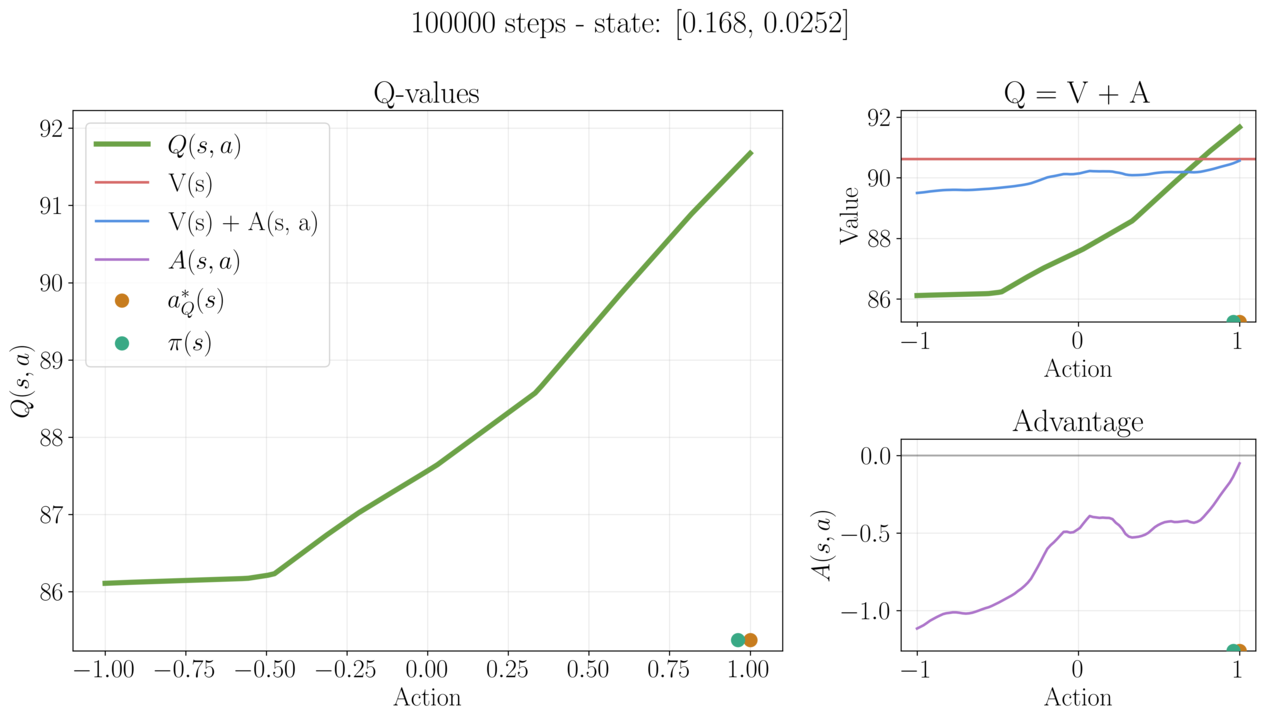
\includegraphics[width=0.8\textwidth]{../figures/afu_mountaincar_action_critic/scaled_02000.png}
        \caption{Évolution des fonctions $Q(s,a)$, $V(s)$, $A(s,a)$ et $V(s)+
        A(s,a)$ en fonction de l'action pour un état critique de MountainCar
        pendant l'entraînement d'AFU. Les courbes montrent la convergence
        progressive vers la forme attendue de la fonction valeur optimale.}
        \label{fig:afu-evolution}
    \end{figure}

    La première catégorie de visualisations se concentre sur l'évolution des
    fonctions critiques pour un état fixé. Ces visualisations montrent comment
    $Q(s,a)$ évolue en fonction de l'action $a$ pour un état $s$ donné. Cette
    approche permet d'observer la forme des fonctions apprises et de détecter
    des comportements anormaux comme des changements brusques localisés ou des
    discontinuités dans les fonctions valeur.

    Pour AFU, ces visualisations révèlent des aspects importants
    de l'apprentissage. La décomposition $Q=V+A$ permet d'observer séparément
    l'évolution de la fonction valeur d'état $V(s)$ et de la fonction
    d'avantage $A(s,a)$. La théorie prévoit que $\max_a A(s,a)$ devrait converger
    vers zéro, ce qui peut être vérifié visuellement. Les visualisations
    montrent également l'évolution de $V(s)+\max_a A(s,a)$, qui devrait converger
    vers $\max_a Q(s,a)$ selon la formulation théorique d'AFU.

    La seconde catégorie de visualisations présente une vue d'ensemble de
    l'espace d'état pendant l'entraînement. Ces visualisations combinent
    plusieurs informations sur un seul graphique : la fonction valeur d'état
    $V(s)$ représentée par un champ de couleur, la politique $\pi(s)$
    visualisée par des flèches indiquant la direction des actions, l'enveloppe
    convexe des états visités dans le replay buffer et les trajectoires
    moyennes suivies par l'agent.

    \begin{figure}[htbp]
        \centering
        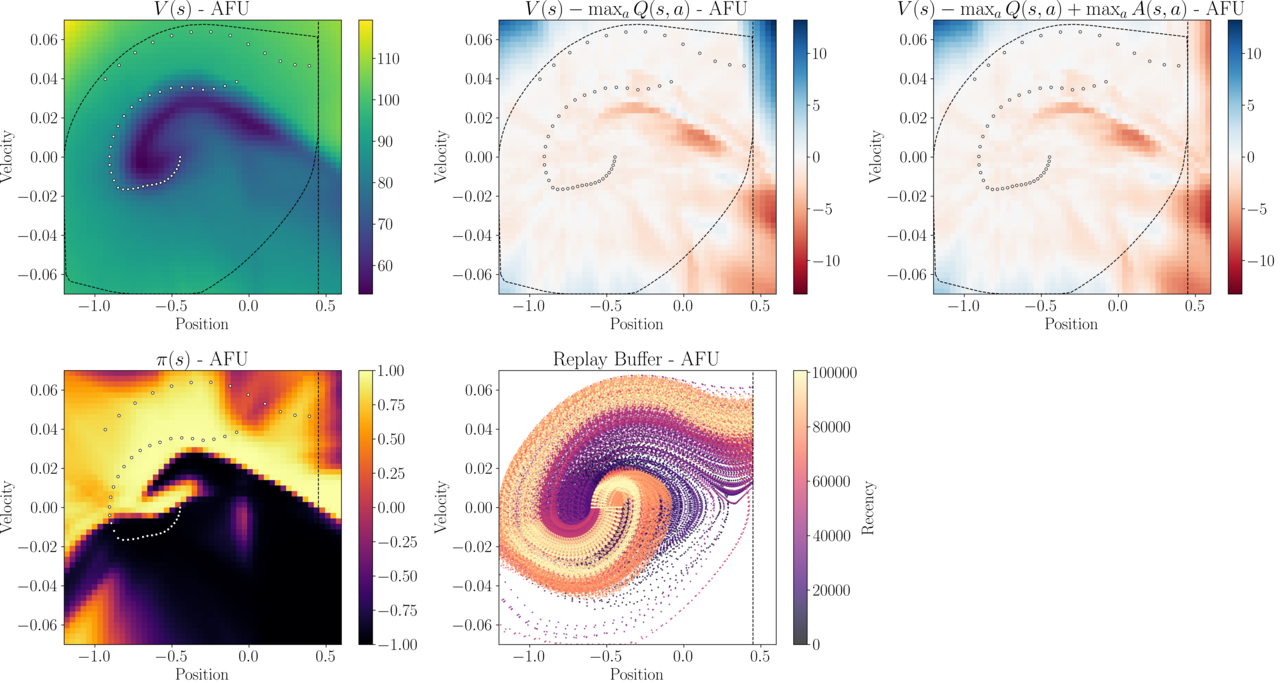
\includegraphics[width=0.8\textwidth]{../figures/afu_mountaincar_critic_policy/scaled_02000.png}
        \caption{Vue d'ensemble de l'espace d'état MountainCar pendant l'entraînement : fonction $V(s)$, politique $\pi(s)$, états du replay buffer, enveloppe convexe (ligne noire) et trajectoires moyennes (points).}
        \label{fig:mountaincar-overview}
    \end{figure}
    
    Un script a également été développé pour calculer l'évolution du biais en
    fonction du temps à chaque point de l'espace d'état. Cette approche aurait
    permis de créer des cartes temporelles du biais montrant comment les
    erreurs d'estimation évoluent et se propagent dans l'espace d'état pendant
    l'apprentissage. Cependant, les calculs de Monte Carlo nécessaires pour
    estimer les vraies valeurs $Q^\pi$ à chaque point et à chaque pas de temps se
    sont révélés prohibitifs en temps de calcul. Les estimations
    initiales suggéraient plusieurs semaines de calcul même avec une grille
    réduite, ce qui a conduit à l'abandon de cette approche.

    \section{La Figure 4 de l'article TQC}

    La Figure 4 de l'article « Controlling Overestimation Bias with Truncated
    Mixture of Continuous Distributional Quantile Critics »
    \cite{kuznetsov2020controllingoverestimationbiastruncated} présente une
    validation expérimentale de TQC sur un MDP jouet simplifié. Cette figure
    constitue une validation importante des contributions de TQC, montrant que
    la troncature des quantiles permet un contrôle précis du biais avec une
    variance réduite par rapport aux méthodes d'ensemble classiques. La
    reproduction de cette expérience a révélé plusieurs problèmes
    méthodologiques qui remettent en question les conclusions originales.

    La reproduction initiale en PyTorch a reproduit des résultats identiques à
    ceux de l'article. Mais la réécriture en JAX a produit des résultats
    différents de ceux reportés dans l'article. De plus, même sur la figure de
    l'article, les valeurs de biais s'étendaient sur une plage de $-100$ à
    $+10000$, alors que les valeurs Q cibles oscillent entre $68$ et $70$
    seulement. Cette disproportion suggérait des problèmes fondamentaux dans le
    processus d'apprentissage. Même des méthodes établies comme l'ensemble
    minimum avec deux critiques (équivalent à TD3) échouaient à apprendre
    correctement sur ce problème simple.

    L'investigation systématique a testé différentes hypothèses : changements
    d'activation (ReLU vers sigmoid), variations d'initialisation,
    modifications des hyperparamètres. Aucune de ces modifications n'a résolu
    les instabilités observées. L'examen des fonctions Q apprises a révélé que
    les réseaux n'arrivaient pas à capturer la forme oscillatoire attendue de
    la fonction de récompense, produisant à la place des approximations
    chaotiques sans relation avec la cible théorique.

    Cette technique, standard en apprentissage par renforcement depuis DQN
    \cite{mnih2015humanlevelcontroldeepreinforcement}, utilise des copies
    lentement mises à jour des paramètres pour calculer les cibles de Bellman.

    Cette analyse complète a fait l'objet d'une documentation détaillée
    disponible sous forme de \href{https://chambaz.xyz/blog/tqc-figure/}{blog
    post}. Le blog post inclut le code de reproduction complet, les analyses
    temporelles étendues et une discussion approfondie des implications pour
    la validation expérimentale en apprentissage par renforcement.

    Le problème jouet a aussi été utilisé pour observer et comprendre le biais
    associé aux différents algorithmes avant de passer sur de vrais
    environnements.

    \section{AFU-TQC}

    AFU utilise un ensemble de réseaux de valeur d'état pour introduire du
    pessimisme dans le calcul des cibles de Bellman. AFU emploie
    $V_{\text{target}} = \min(V_1, V_2)$ pour réduire la surestimation. Cette
    approche, bien que simple, limite les capacités de contrôle du biais, en
    particulier si on la compare à des méthodes existantes plus sophistiquées
    comme TQC.

    TQC démontre qu'un contrôle précis du niveau de pessimisme peut être obtenu
    en manipulant le nombre de quantiles supprimés dans la distribution
    tronquée. Cette flexibilité permet d'ajuster le compromis
    biais-variance selon les besoins de l'environnement. L'hypothèse centrale
    d'AFU-TQC était que cette capacité de contrôle fin pourrait bénéficier à
    AFU, dans des environnements où le niveau optimal de pessimisme diffère de
    celui obtenu par la simple minimisation d'ensemble.

    L'intégration de TQC dans AFU révèle rapidement des incompatibilités
    fondamentales avec l'architecture des fonctions de perte jointes. AFU
    optimise simultanément les réseaux $Q$, $V$ et $A$ à travers une fonction
    de perte unifiée qui garantit les contraintes $V + A = Q$ et $\max_a A(s,a)
    \leq 0$.

    TQC opère sur des distributions de quantiles indépendantes
    qui nécessitent une régression quantile avec des fonctions de perte
    asymétriques. L'intégration naïve de ces deux approches crée des conflits
    dans les objectifs d'optimisation : les contraintes structurelles d'AFU
    deviennent difficiles à maintenir quand les cibles proviennent de
    distributions tronquées.

    Le problème principal réside dans la nature des cibles d'apprentissage.
    Pour appliquer les mécanismes de troncature de TQC, il faut que $V$ soit
    représenté de manière distributionnelle. Cependant, dans AFU, $V + A$ doit
    apprendre à estimer $Q$, qui dans l'approche standard n'est pas distribué.
    Cette asymétrie crée une incompatibilité : comment $V$ peut-il apprendre à
    partir d'une cible distributionnelle ?

    Deux approches ont été explorées pour résoudre cette incompatibilité. La
    première tentative consistait à rendre toutes les composantes
    distributionnelles :

    \begin{itemize}
      \item $V_\psi : \mathcal{S} \rightarrow \mathbb{R}^M$ produit $M$ quantiles d'état ;
      \item $A_\phi : \mathcal{S} \times \mathcal{A} \rightarrow \mathbb{R}^M$ produit $M$ quantiles d'avantage ;
      \item $Q_\theta : \mathcal{S} \times \mathcal{A} \rightarrow \mathbb{R}^M$ produit $M$ quantiles de valeur.
    \end{itemize}

    Cette approche s'est révélée instable en pratique, les distributions
    apprises par $V$ et $A$ ne convergeant pas vers des formes cohérentes.

    L'approche finalement retenue utilise une architecture hybride :

    \begin{itemize}
      \item $V_\psi : \mathcal{S} \rightarrow \mathbb{R}$ produit un scalaire ;
      \item $A_\phi : \mathcal{S} \times \mathcal{A} \rightarrow \mathbb{R}$ produit un scalaire ;
      \item $Q_\theta : \mathcal{S} \times \mathcal{A} \rightarrow \mathbb{R}^M$ produit $M$ quantiles de valeur.
    \end{itemize}

    $Q_\theta$ apprend alors la distribution des $Q$ issue de l'environnement.
    $V_\psi + A_\phi$ apprend sous les contraintes de $A_\phi<0$ et $V_\psi$
    une borne serrée à apprendre l'espérance de $Q$ tronquée selon la méthode
    de TQC. $V_\psi$ appris est alors pessimiste et ce pessimisme impacte
    directement la distribution sur laquelle $Q$ apprend. $Q_\theta$ apprend
    donc une
    distribution pessimiste, qui permet l'implémentation voulue.

    Mais l'évaluation d'AFU-TQC sur MountainCar Continuous a révélé des
    performances décevantes. L'agent peinait à converger vers une politique
    efficace, avec des courbes d'apprentissage erratiques et une performance
    finale inférieure à AFU standard.

    L'hypothèse pour la cause de l'échec a été la suivante : l'architecture
    hybride introduit une complexité algorithmique disproportionnée par rapport
    aux bénéfices attendus. Les hyperparamètres supplémentaires (nombre de
    quantiles, niveau de troncature) augmentent l'espace de recherche sans
    garantie de convergence.

    L'évolution de la compréhension de AFU a laissé penser que le paramètre de
    contrôle $\rho$ de AFU, utilisé initialement pour imposer la contrainte de
    $V(s)$ comme borne serrée de $\max_a Q(s, a)$, pouvait être utilisé comme un
    paramètre de contrôle sur le biais. $\rho$ impose une pression vers le bas
    sur $V(s)$, mais avec un $\rho$ élevé, $V(s)$ prend une valeur plus faible,
    ce qui peut être perçu comme un moyen d'être pessimiste sur la valeur de
    $V(s')$.

    Cette analyse a conduit à l'abandon d'AFU-TQC au profit d'approches plus
    directes pour étudier le biais dans AFU.

    \section{Mesure du biais}

    L'évaluation rigoureuse du biais d'estimation en apprentissage par
    renforcement nécessite la comparaison entre les valeurs apprises par les
    critiques neuronaux $Q_\theta(s,a)$ et les vraies valeurs $Q^\pi(s,a)$
    associées à la politique courante. Cette comparaison directe présente un
    défi fondamental : comment estimer précisément $Q^\pi(s,a)$ pour une
    politique donnée dans des environnements où la solution analytique n'existe
    pas ?

    La définition théorique $Q^\pi(s,a) = \mathbb{E}_\pi[G_t | S_t = s, A_t =
    a]$ où $G_t = \sum_{k=0}^{\infty} \gamma^k R_{t+k+1}$ implique le calcul
    d'une espérance sur toutes les trajectoires possibles à partir d'un couple
    état-action donné. Dans des environnements stochastiques ou avec des
    espaces d'état-action continus, cette espérance ne peut être calculée
    analytiquement.

    Le problème se complexifie dans le contexte de l'apprentissage par
    renforcement off-policy, où la politique $\pi$ évolue constamment pendant
    l'entraînement. Il devient nécessaire d'estimer $Q^\pi$ pour chaque
    politique intermédiaire $\pi_t$ rencontrée au cours de l'apprentissage, ce
    qui multiplie les calculs requis.

    Pour formaliser l'approche Monte Carlo, définissons $Q^\pi(s,a)$ comme la
    valeur exacte d'action sous la politique $\pi$ :

    $$
    Q^\pi(s,a) = \mathbb{E}_\pi\left[\sum_{k=0}^{\infty} \gamma^k R_{t+k+1} \mid S_t = s, A_t = a\right].
    $$

    L'estimateur Monte Carlo $\hat{Q}^\pi_N(s,a)$ approche cette espérance par
    la moyenne empirique de $N$ trajectoires indépendantes :

    $$
    \hat{Q}^\pi_N(s,a) = \frac{1}{N} \sum_{i=1}^{N} G^{(i)}_t,
    $$

    où $G^{(i)}_t$ représente le retour cumulé de la $i$-ème trajectoire commençant par l'état $s$ et l'action $a$.

    La méthodologie développée opère en plusieurs étapes pour estimer
    empiriquement le biais à différents moments de l'entraînement. À chaque
    évaluation, l'algorithme échantillonne uniformément $M$ couples $(s_j,
    a_j)$ depuis le replay buffer de l'agent. Cette approche assure que les
    points d'évaluation correspondent aux régions de l'espace d'état-action
    visitées pendant l'apprentissage. Il faut, pour chaque couple
    échantillonné, déterminer le pas de temps $t_j$ auquel cette transition a
    été observée dans l'épisode correspondant. Cette information temporelle est
    cruciale pour initialiser correctement l'environnement lors des simulations
    Monte Carlo.

    Pour chaque couple $(s_j, a_j, t_j)$, l'algorithme génère $N$ trajectoires
    indépendantes selon le protocole suivant, en le répétant jusqu'à un état
    terminal :

    \begin{itemize}
      \item sélection d'une action pour l'état donné par la politique courante;
      \item retour de l'environnement de l'état suivant et de la récompense.
    \end{itemize}

    Cette procédure garantit que chaque trajectoire commence dans les
    conditions $(s_j, a_j, t_j)$ observées pendant l'entraînement, puis suit la
    politique courante $\pi$ jusqu'à la terminaison de l'épisode.

    Une fois les estimations Monte Carlo $\hat{Q}^\pi_N(s_j, a_j)$ calculées et
    les valeurs du critique $Q_\theta(s_j, a_j)$ extraites, le biais empirique
    est quantifié par :

    $$
    \text{Biais} = \frac{1}{M} \sum_{j=1}^M (Q_\theta(s_j, a_j) - \hat{Q}^\pi_N(s_j, a_j)).
    $$

    La méthode Monte Carlo présente une complexité $O(M \times N \times L)$ où
    $M$ est le nombre de couples état-action évalués, $N$ le nombre de
    trajectoires par couple et $L$ la longueur moyenne des épisodes. Pour des
    évaluations fréquentes pendant l'entraînement, cette complexité devient
    prohibitive.

    Les contraintes pratiques ont conduit aux compromis suivants :

    \begin{itemize}
      \item évaluation tous les 1000 pas d'entraînement;
      \item $M = 20$ couples état-action par évaluation;
      \item $N = 50$ trajectoires par couple.
    \end{itemize}

    L'échantillonnage depuis le replay buffer introduit un biais vers les
    régions fréquemment visitées. Cette limitation est acceptable car
    l'objectif est d'évaluer le biais dans les régions utilisées pour
    l'apprentissage.

    Cette méthodologie, bien que coûteuse, fournit des mesures empiriques
    robustes du biais d'estimation, permettant l'analyse comparative détaillée
    des différents algorithmes présentée dans la section suivante.

    \section{Résultats expérimentaux}

    L'évaluation empirique du biais d'estimation sur MountainCar Continuous
    révèle des comportements complexes qui remettent en question certaines
    intuitions théoriques sur la relation entre contrôle du biais et
    performance d'apprentissage. Les mesures Monte Carlo permettent une analyse
    quantitative précise du biais pour chaque algorithme et de l'efficacité des
    différents mécanismes de contrôle.

    L'analyse commence par l'étude de MSAC (Mean SAC), une variante de SAC
    utilisant la moyenne des critiques au lieu du minimum pour le calcul des
    cibles. Cette modification élimine le mécanisme pessimiste standard de SAC,
    fournissant une référence pour mesurer l'impact des corrections de biais.

    Les résultats révèlent une dynamique temporelle contre-intuitive. MSAC
    présente un biais systématiquement inférieur à celui de SAC, l'inverse de ce à quoi on devrait s'attendre car SAC devrait être plus
    pessimiste que MSAC.

    Cette inversion suggère des interactions complexes entre plusieurs
    mécanismes. Le pessimisme appliqué aux cibles de Bellman influence
    directement la politique apprise, qui à son tour modifie la distribution
    d'échantillonnage du replay buffer. Ces changements de distribution
    affectent les cibles futures, créant une boucle de rétroaction qui peut
    conduire à des dynamiques d'évolution du biais non triviales. L'observation
    remet en question l'hypothèse selon laquelle un contrôle statique
    du biais (par exemple, un minimum fixe) produit des effets prévisibles sur
    l'ensemble de l'apprentissage.


    \begin{figure}[htbp]
        \centering
        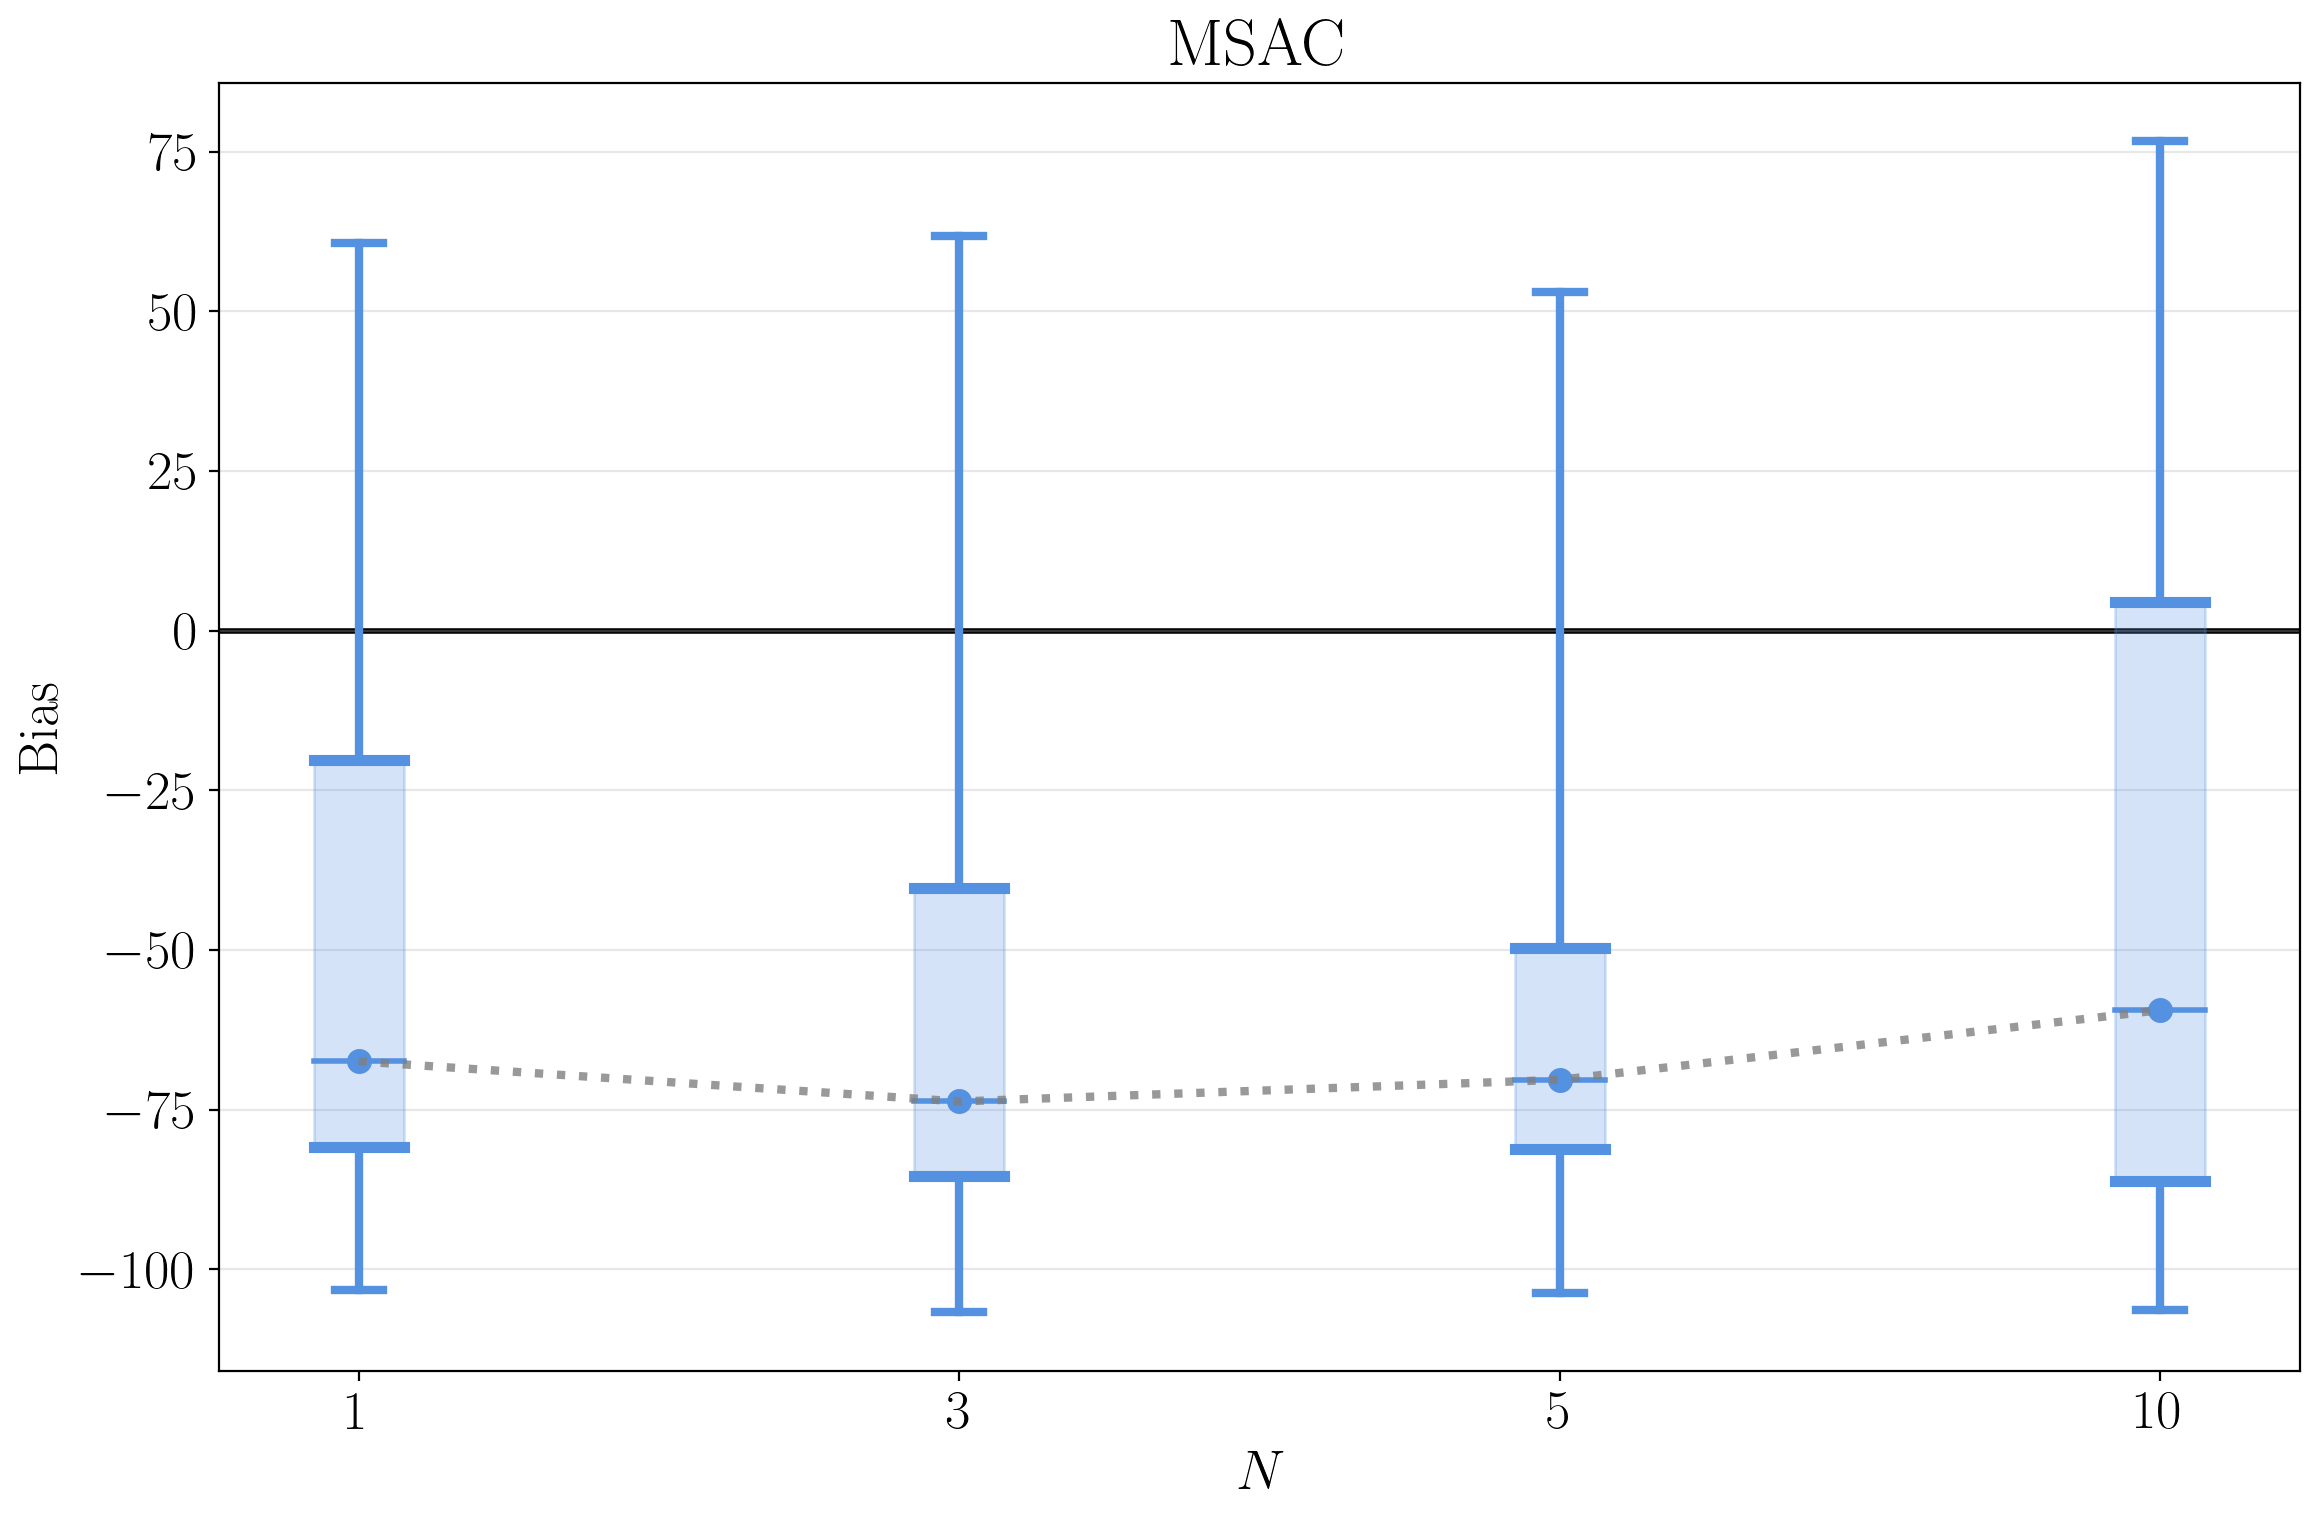
\includegraphics[width=0.4\textwidth]{../figures/env_param_msac.png}
        \quad
        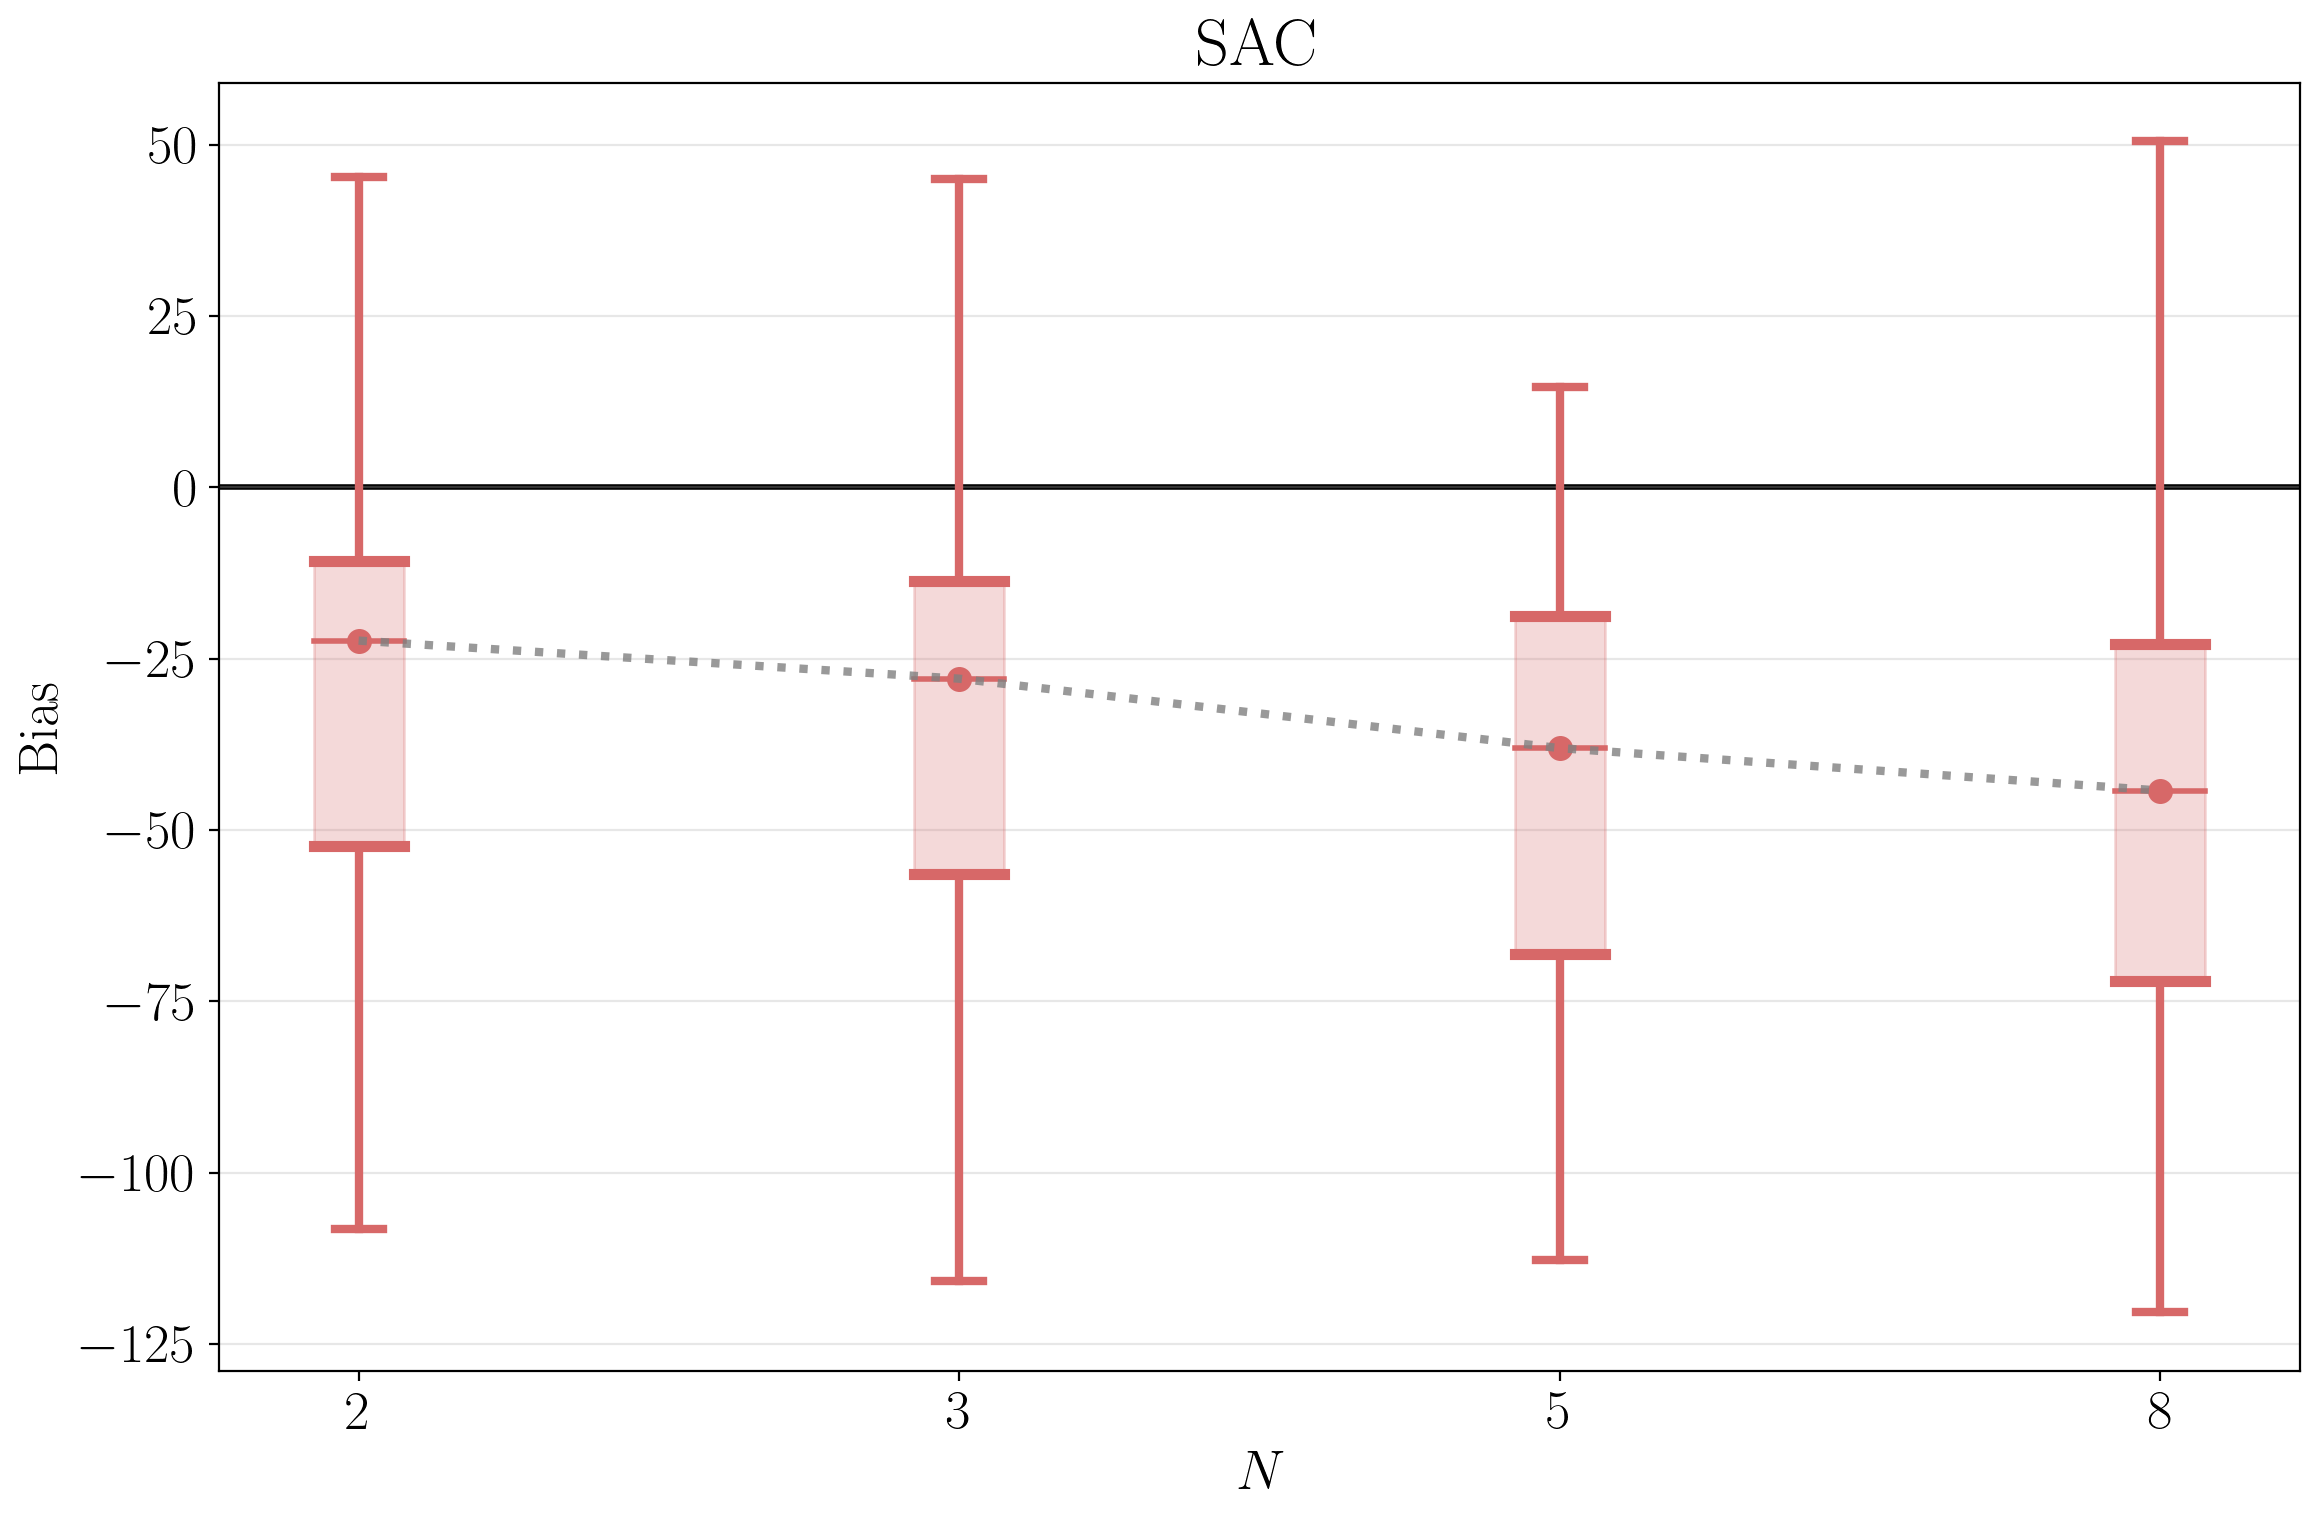
\includegraphics[width=0.4\textwidth]{../figures/env_param_sac.png}

        \vspace{0.5cm}

        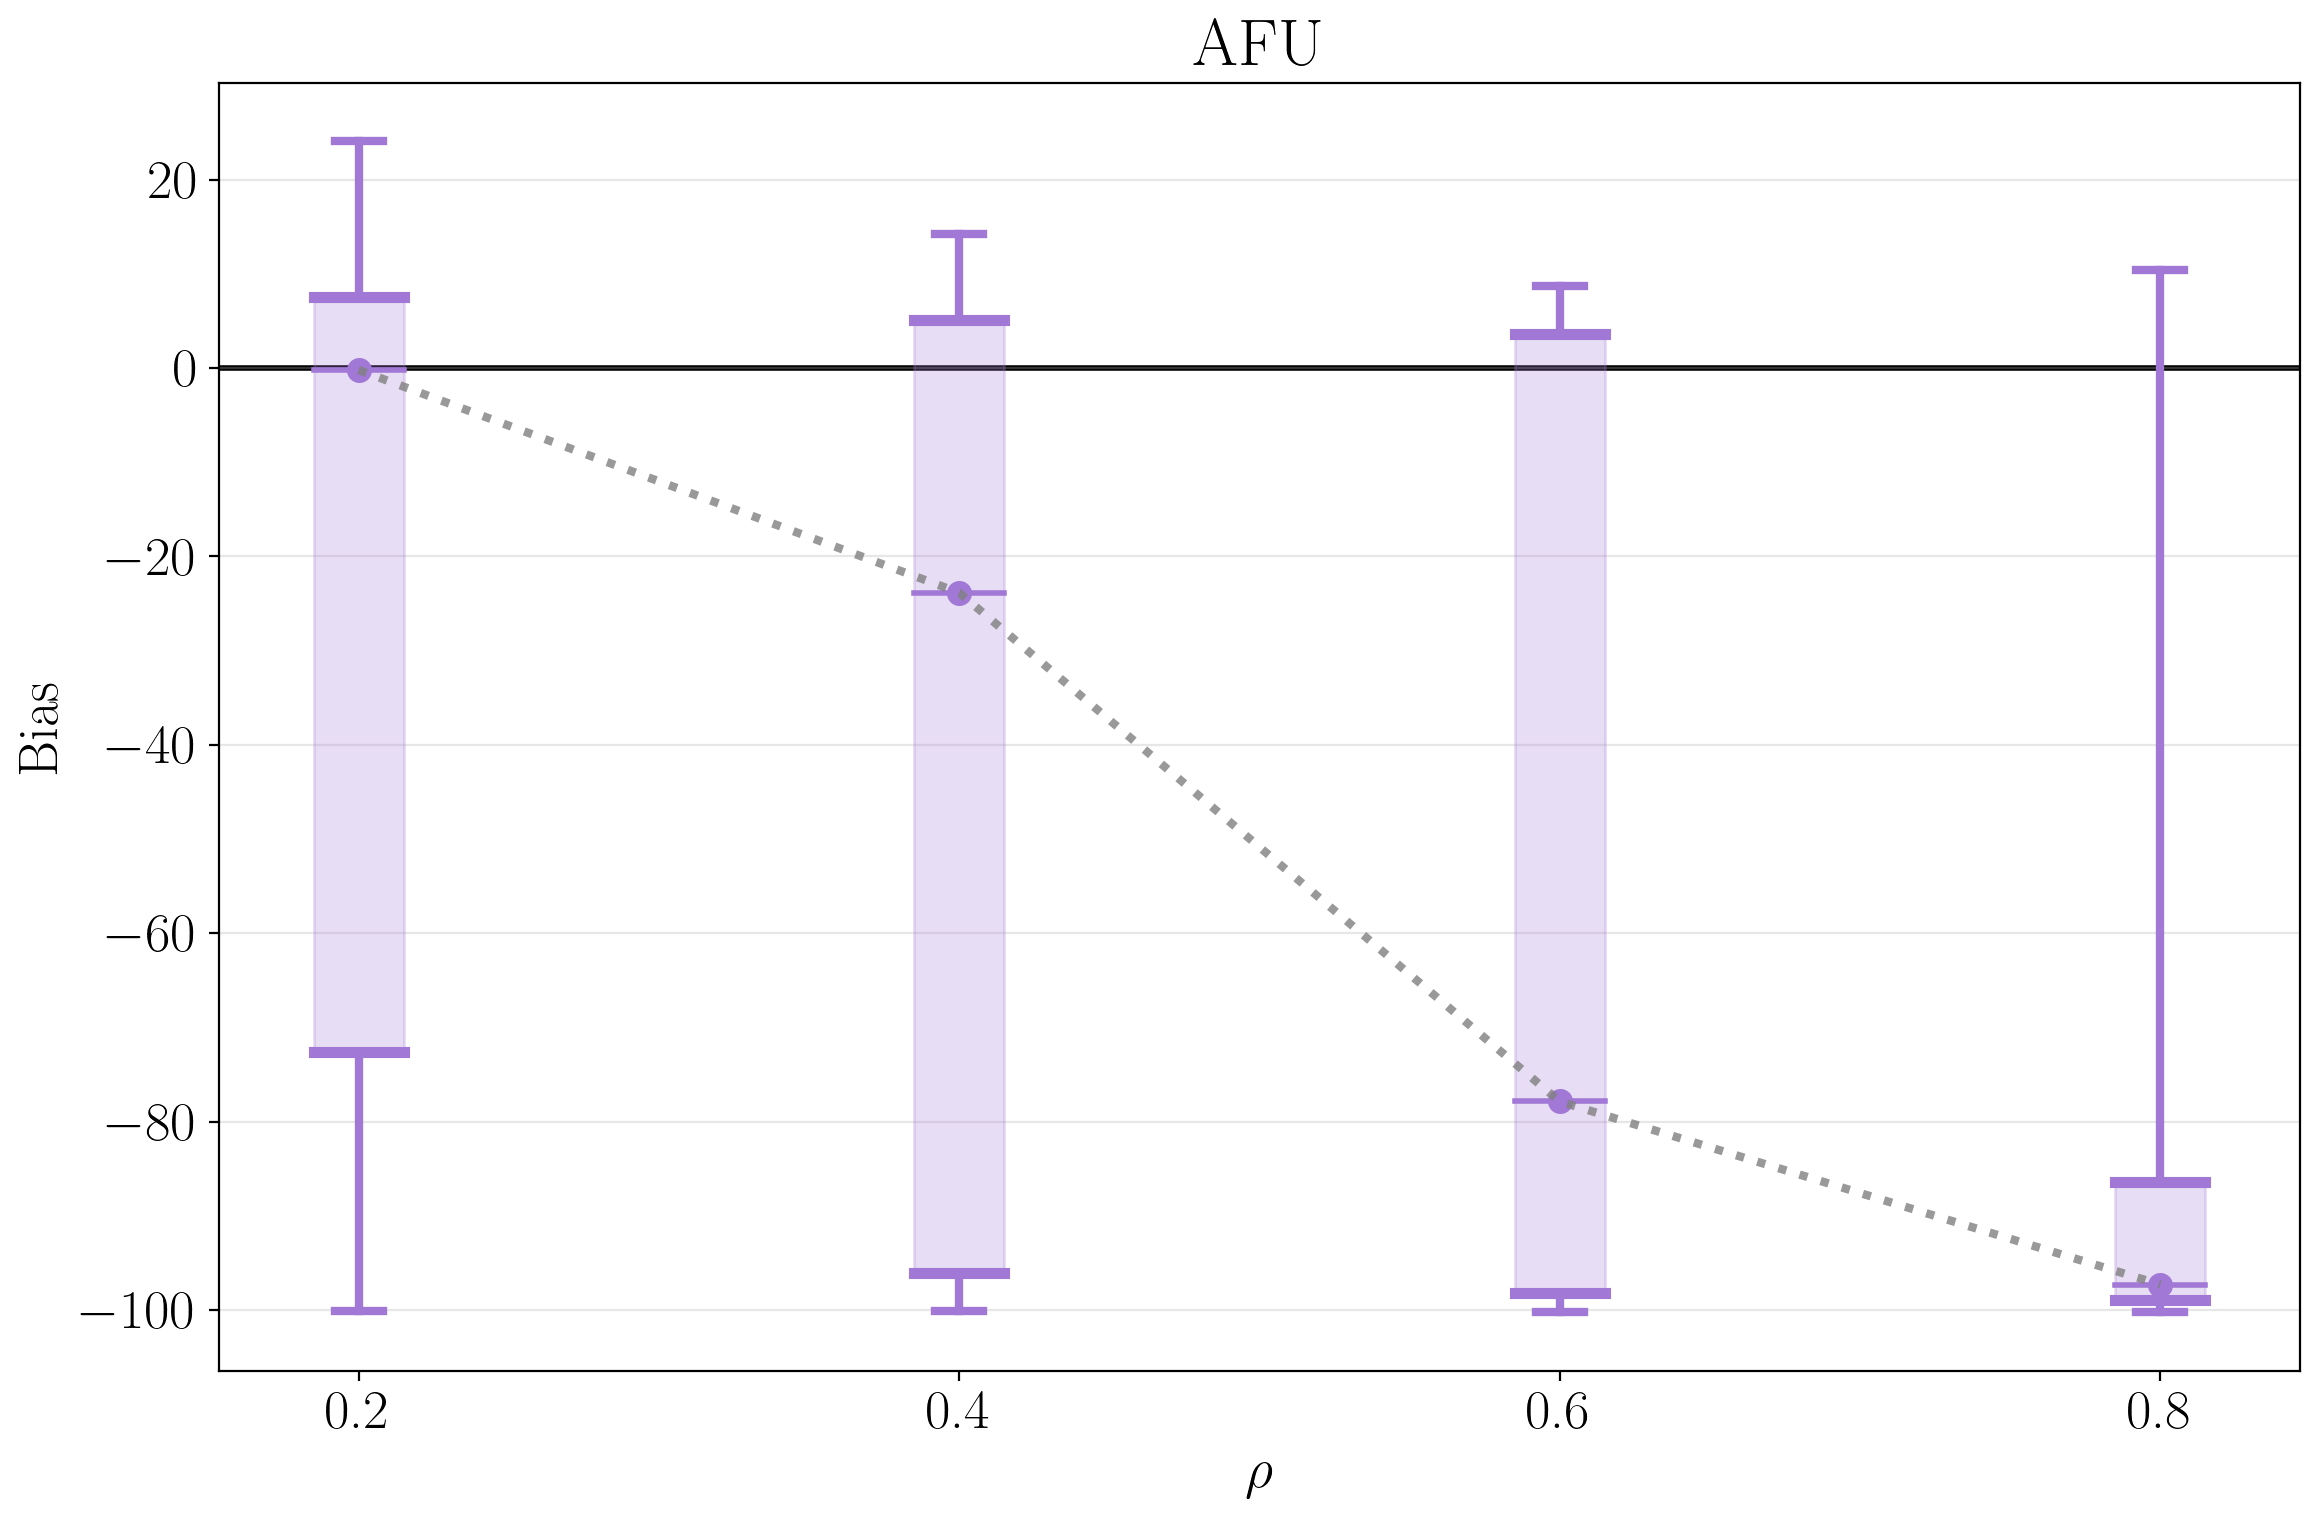
\includegraphics[width=0.4\textwidth]{../figures/env_param_afu.png}
        \quad
        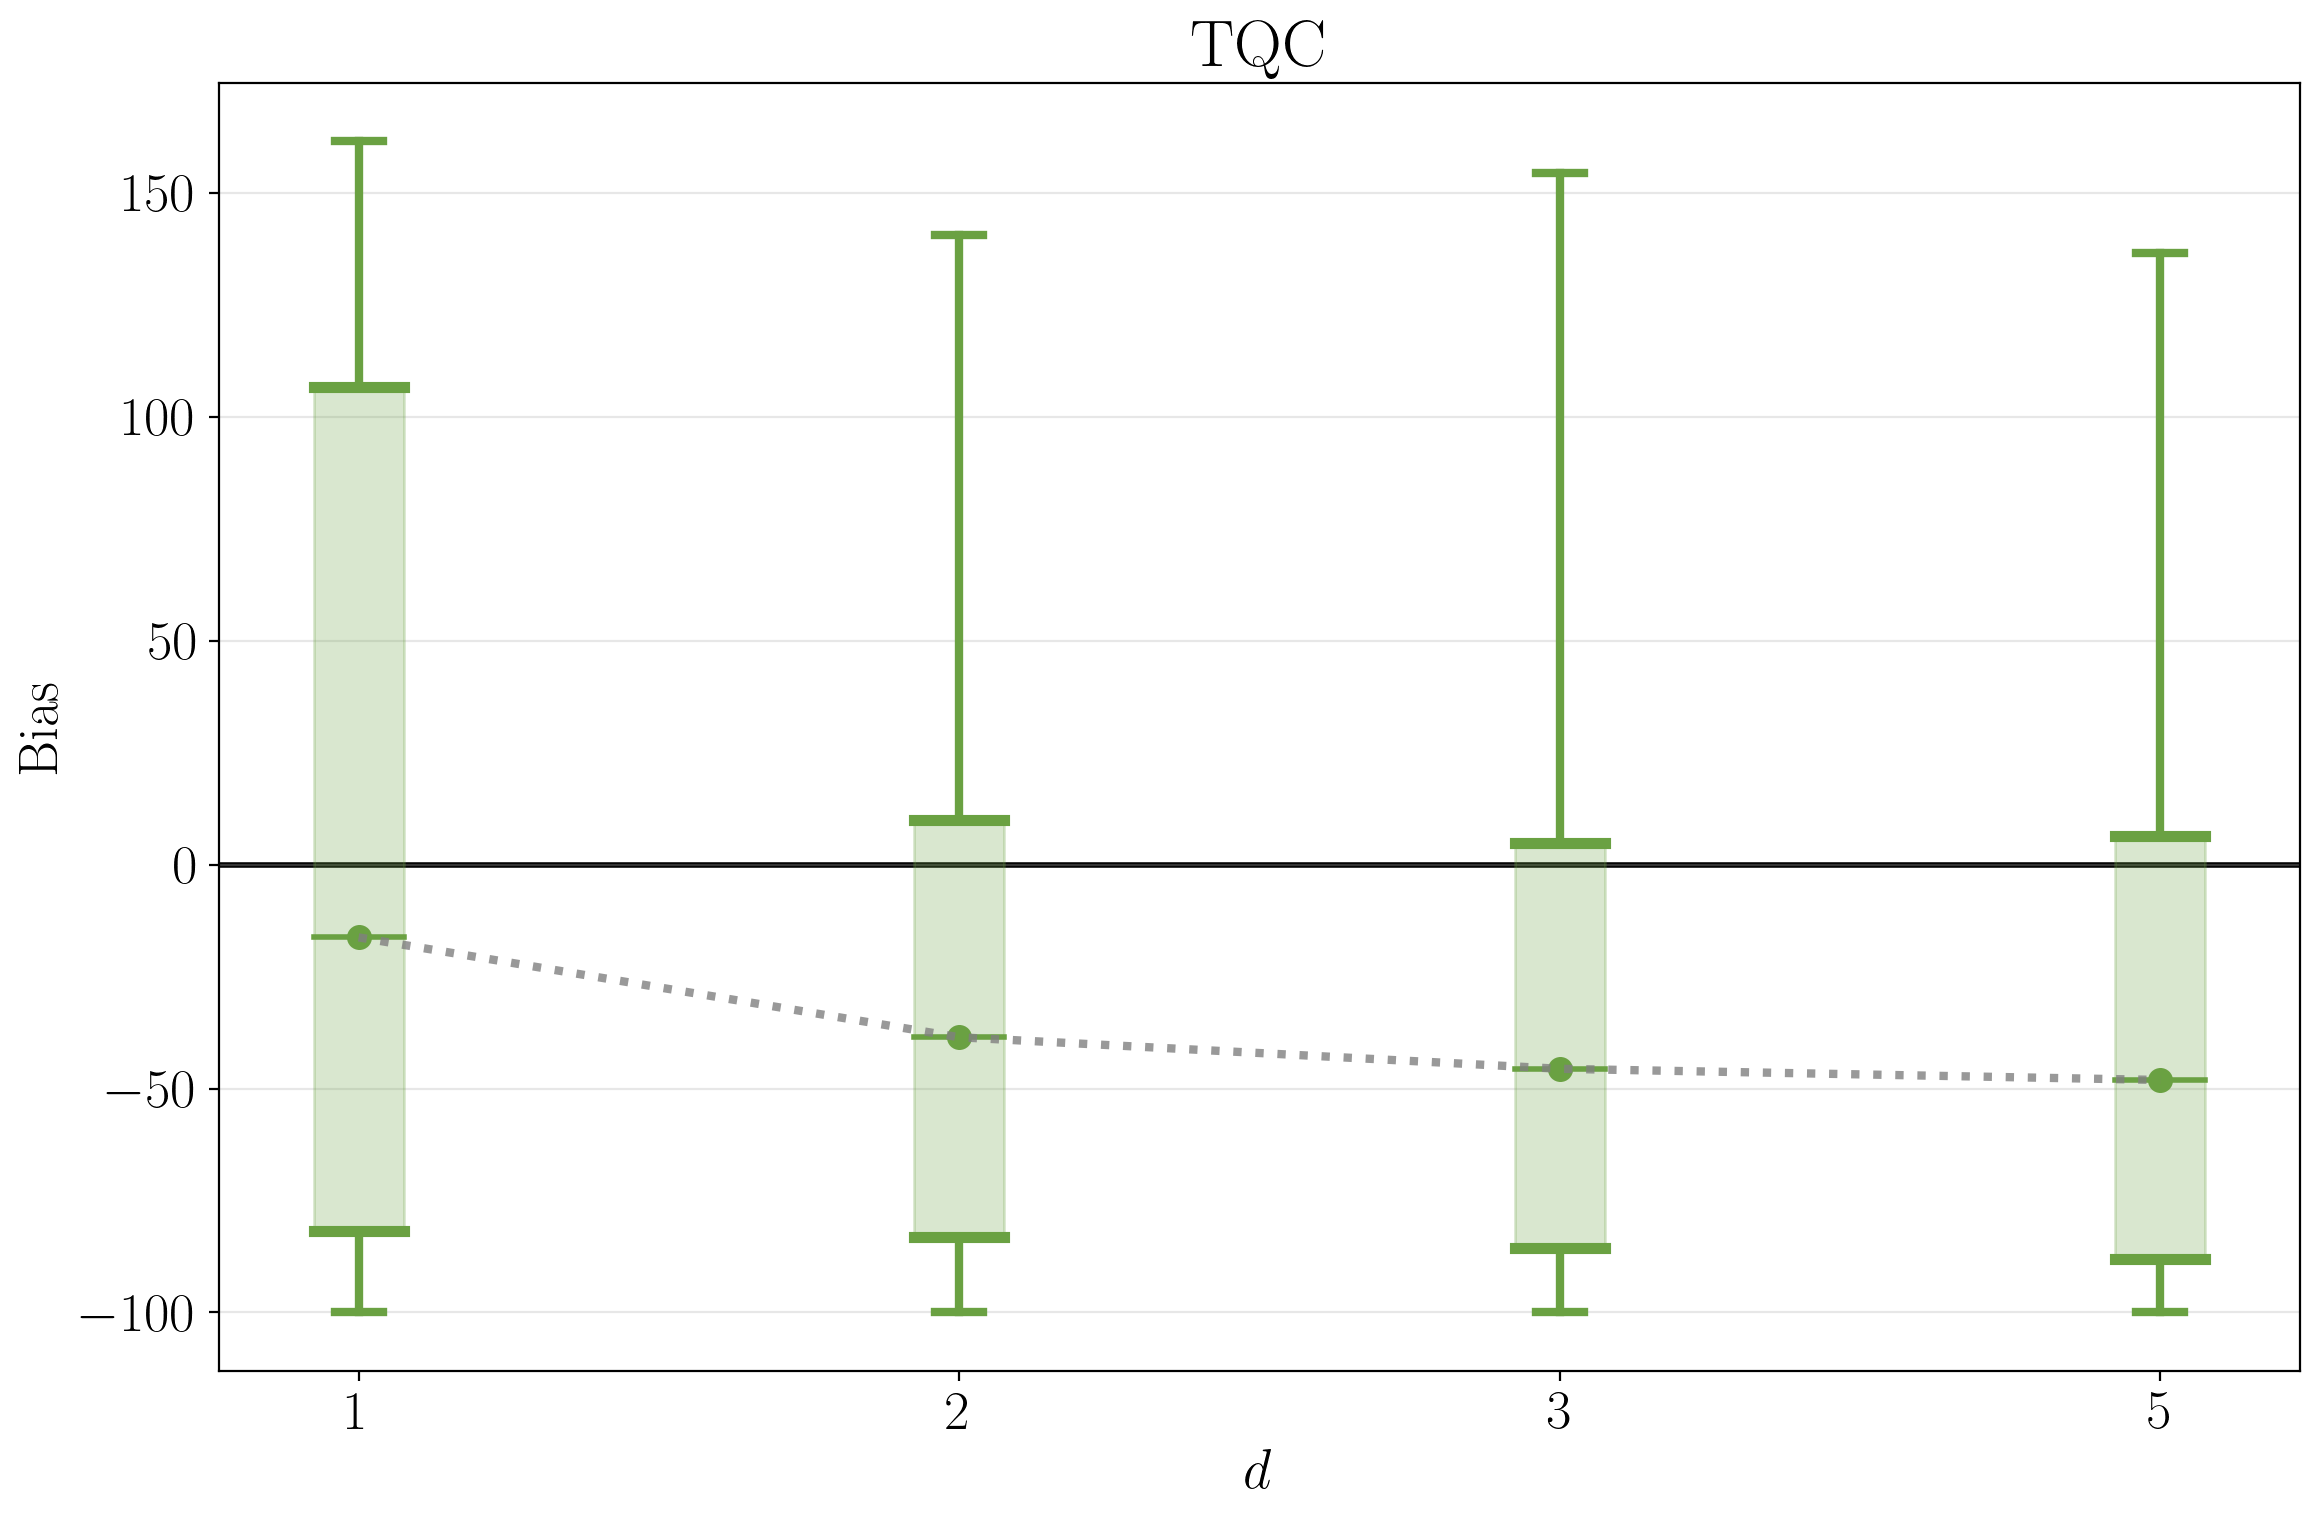
\includegraphics[width=0.4\textwidth]{../figures/env_param_tqc.png}
        
        \vspace{0.5cm}

        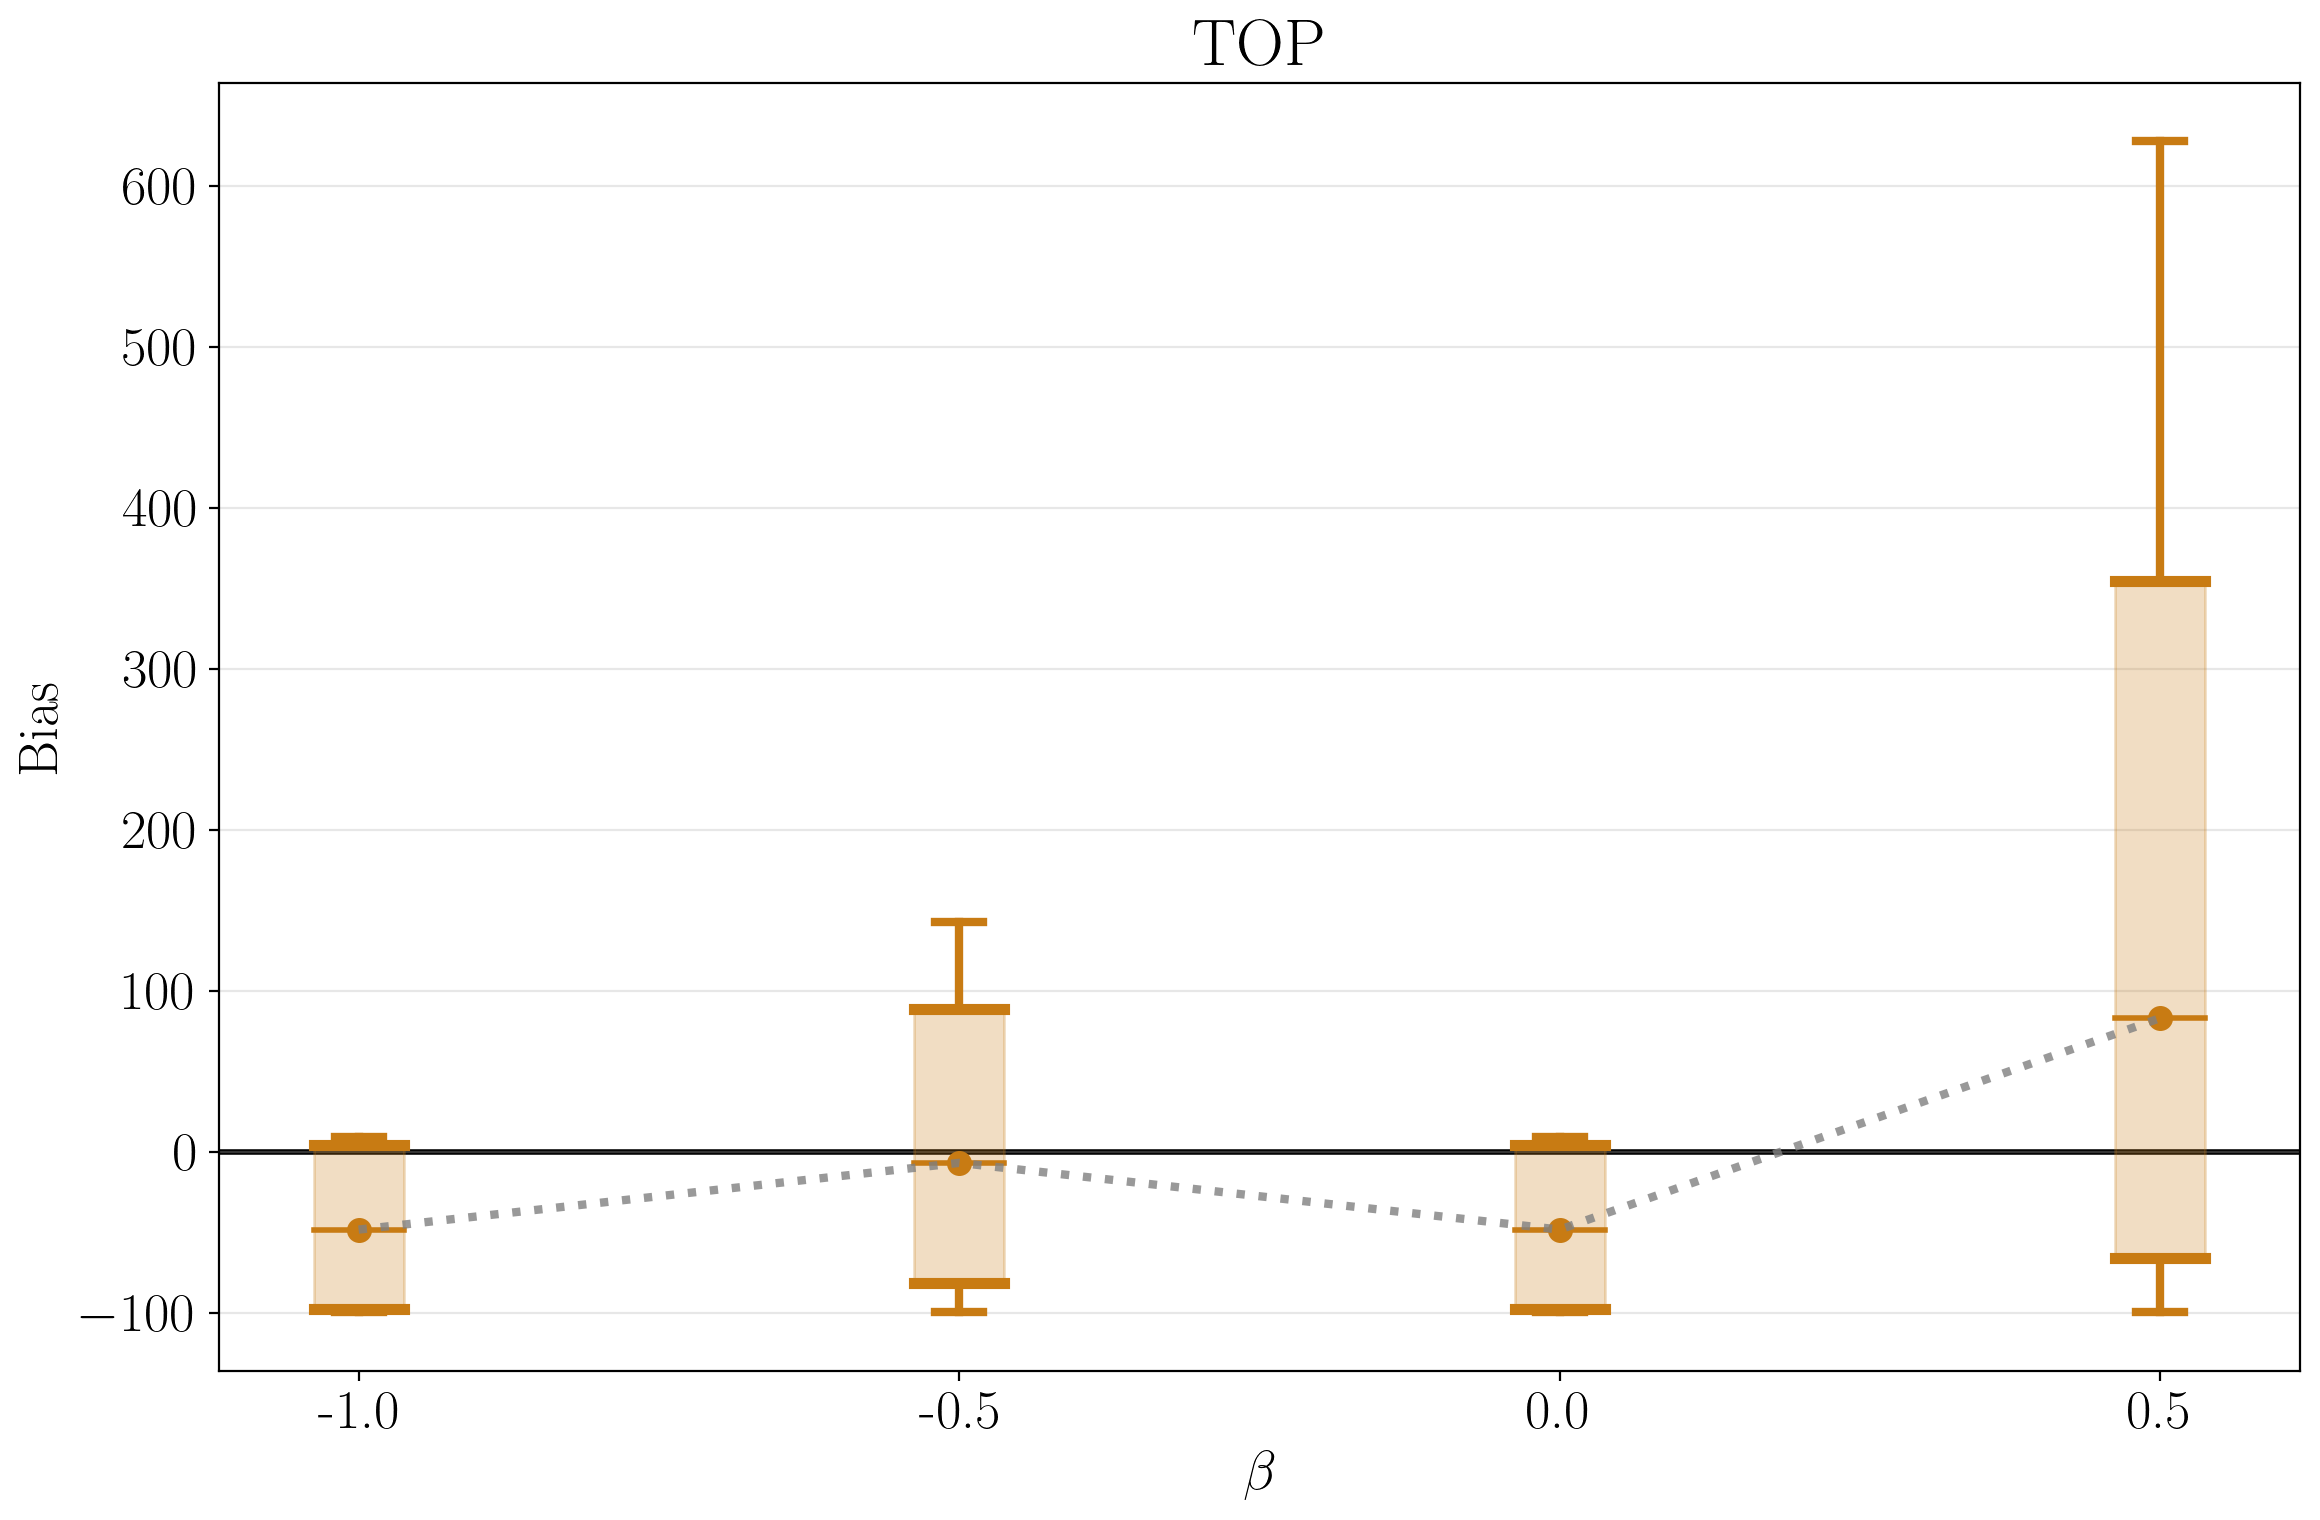
\includegraphics[width=0.4\textwidth]{../figures/env_param_top.png}
        
        \caption{Boîtes à moustaches montrant l'impact du paramètre qui contrôle le pessimisme sur le biais mesuré empiriquement sur MountainCar Continuous. Chaque boîte montre MIN/Q3/IQM/Q1/MAX. Dans l'ordre : MSAC, SAC, AFU, TQC, TOP.}
        \label{fig:bias-measurements}
    \end{figure}

    SAC avec différentes tailles d'ensemble présente un comportement plus
    prévisible et cohérent avec la théorie. L'augmentation du nombre de
    critiques dans l'ensemble amplifie l'effet du mécanisme pessimiste : plus
    l'ensemble est large, plus la valeur minimale sélectionnée tend à être
    faible, induisant un biais négatif plus prononcé.

    Cette relation monotone entre la taille de l'ensemble et le niveau de
    pessimisme confirme l'efficacité du mécanisme TD3/SAC pour contrôler le
    biais de maximisation. L'évolution temporelle du biais reste relativement
    stable, sans les inversions observées avec MSAC, suggérant que le mécanisme
    du minimum d'ensemble produit des effets plus robustes que la moyenne.

    AFU présente le comportement le plus intéressant parmi tous les algorithmes
    testés. Le paramètre $\rho$ exerce un impact important sur le niveau de
    biais observé, avec une relation claire et monotone : de petites valeurs de
    $\rho$ correspondent à une faible pression pessimiste et produisent un
    biais positif, tandis que de grandes valeurs de $\rho$ imposent une forte
    pression pessimiste et génèrent un biais négatif substantiel. Cette
    observation confirme et étend l'hypothèse d'utilisation de $\rho$ comme
    mécanisme de contrôle du biais dans AFU. AFU présente la plage de contrôle
    la plus étendue parmi tous les algorithmes testés.

    Cette amplitude de contrôle suggère que le mécanisme de AFU pour gérer le
    biais diffère des approches par ensemble ou troncature. La nature continue
    et directe de l'influence de $\rho$ sur les fonctions de perte pourrait
    expliquer cette efficacité supérieure.

    TQC démontre un contrôle précis du biais grâce à son paramètre de
    troncature. L'augmentation du nombre de quantiles supprimés produit un
    effet pessimiste graduel et prévisible, permettant un ajustement fin du
    compromis biais-variance. Cette granularité de contrôle représente un
    avantage technique par rapport aux méthodes d'ensemble.

    TOP révèle des comportements plus complexes selon la valeur du paramètre
    $\beta$. Pour $\beta$ < 0 (pessimisme), l'algorithme contrôle efficacement
    la surestimation avec des résultats similaires à TQC. Cependant, pour
    $\beta$ > 0 (optimisme), des phénomènes de surestimation apparaissent et se
    propagent par amplification du biais de maximisation. Ces surestimations
    confirment les risques des approches optimistes en présence de bruit
    d'estimation important.

    L'observation la plus étonnante concerne la relation entre contrôle du
    biais et qualité de l'apprentissage. Contrairement aux attentes théoriques,
    l'examen des courbes de performance révèle des motifs chaotiques qui ne
    sont pas corrélés avec les niveaux de biais mesurés.

    \begin{figure}[htbp]
        \centering
        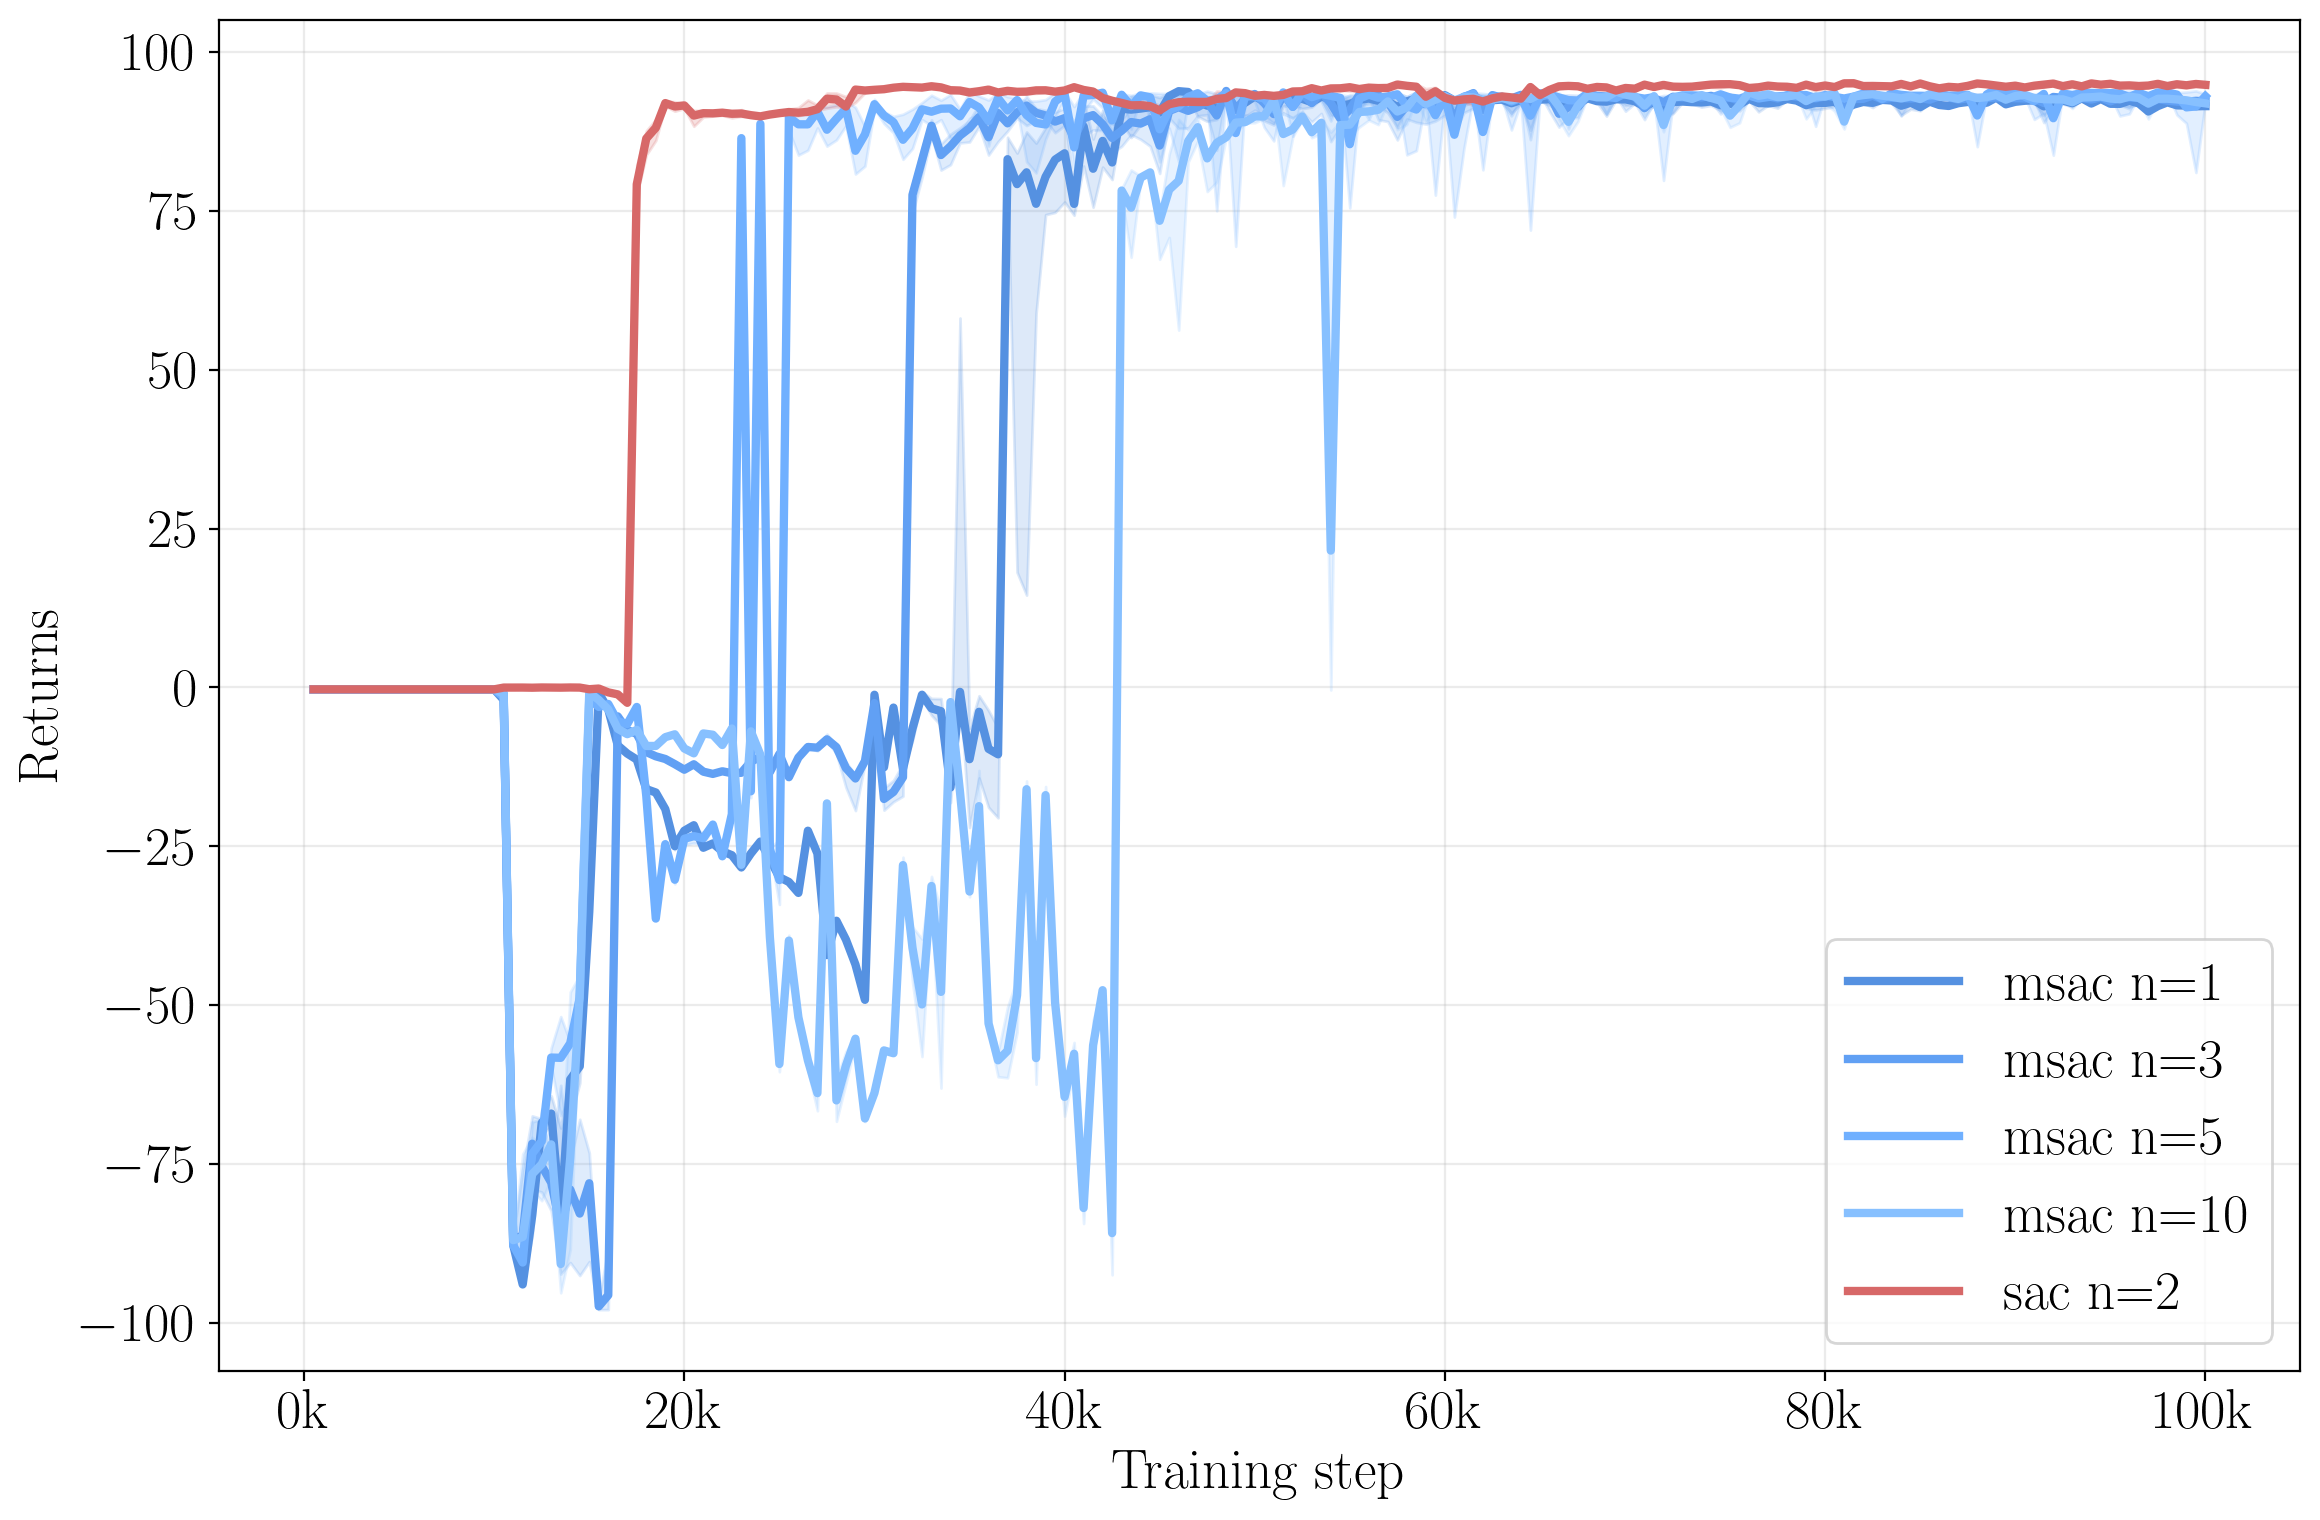
\includegraphics[width=0.3\textwidth]{../figures/env_returns_msac.png}
        \hfill
        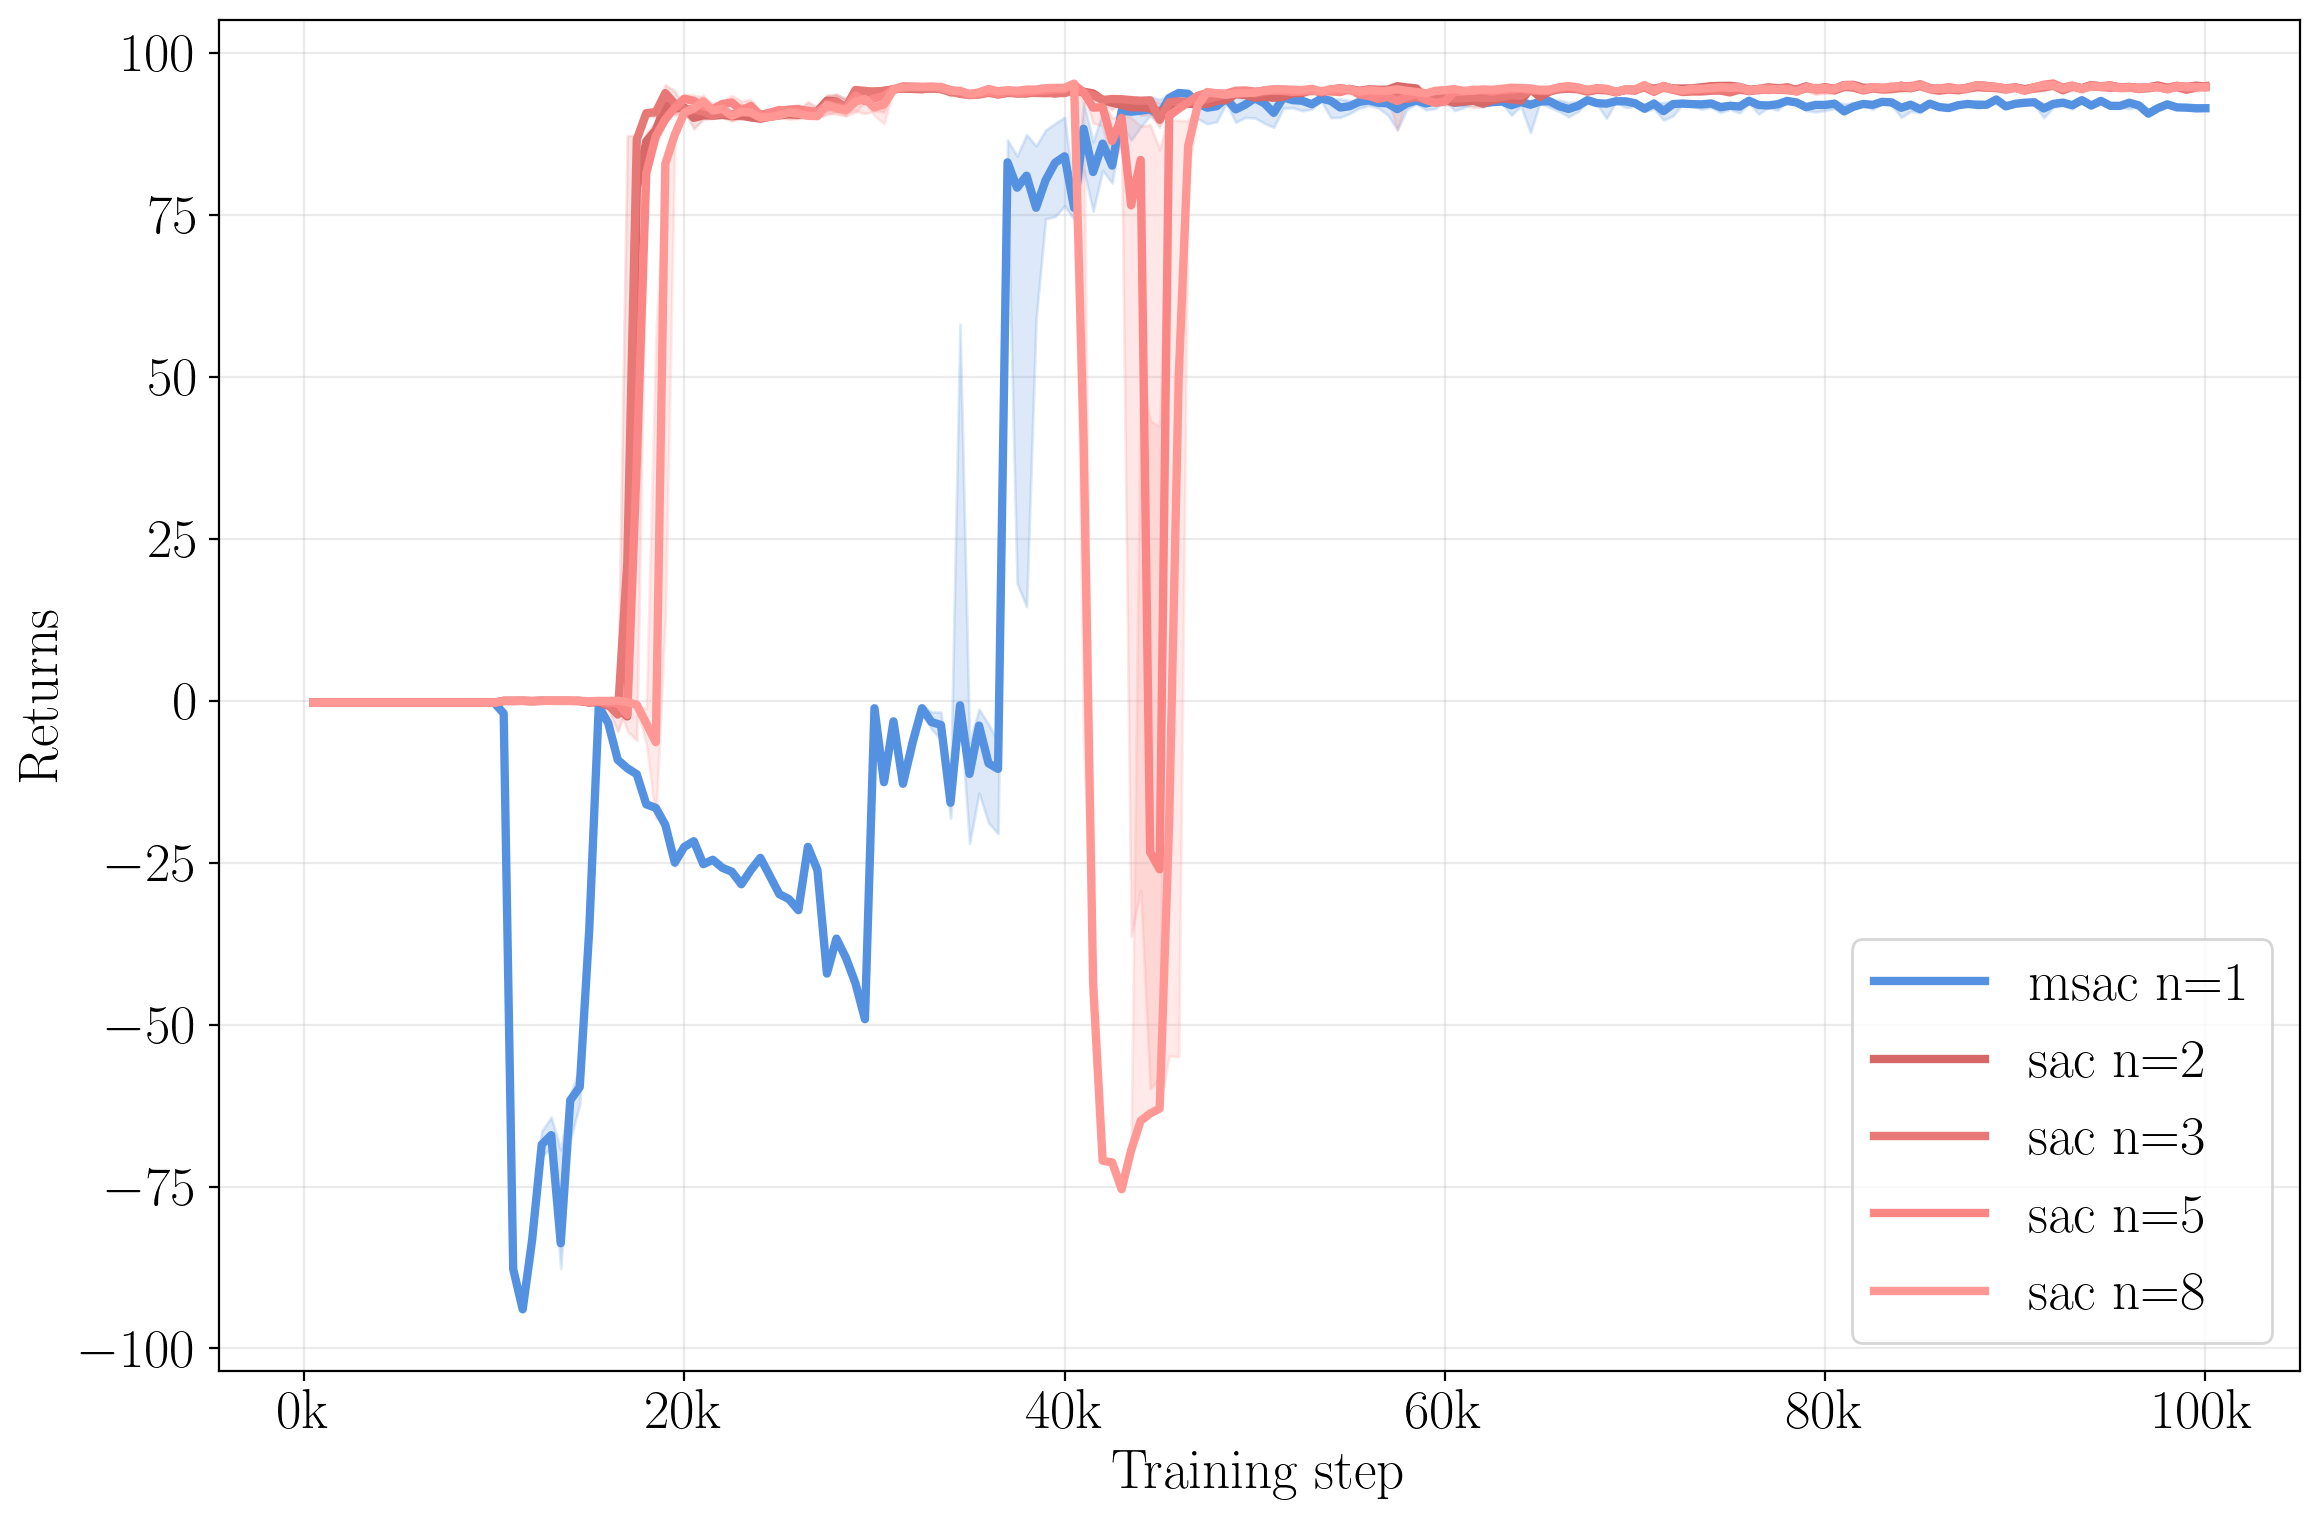
\includegraphics[width=0.3\textwidth]{../figures/env_returns_sac.png}
        \hfill
        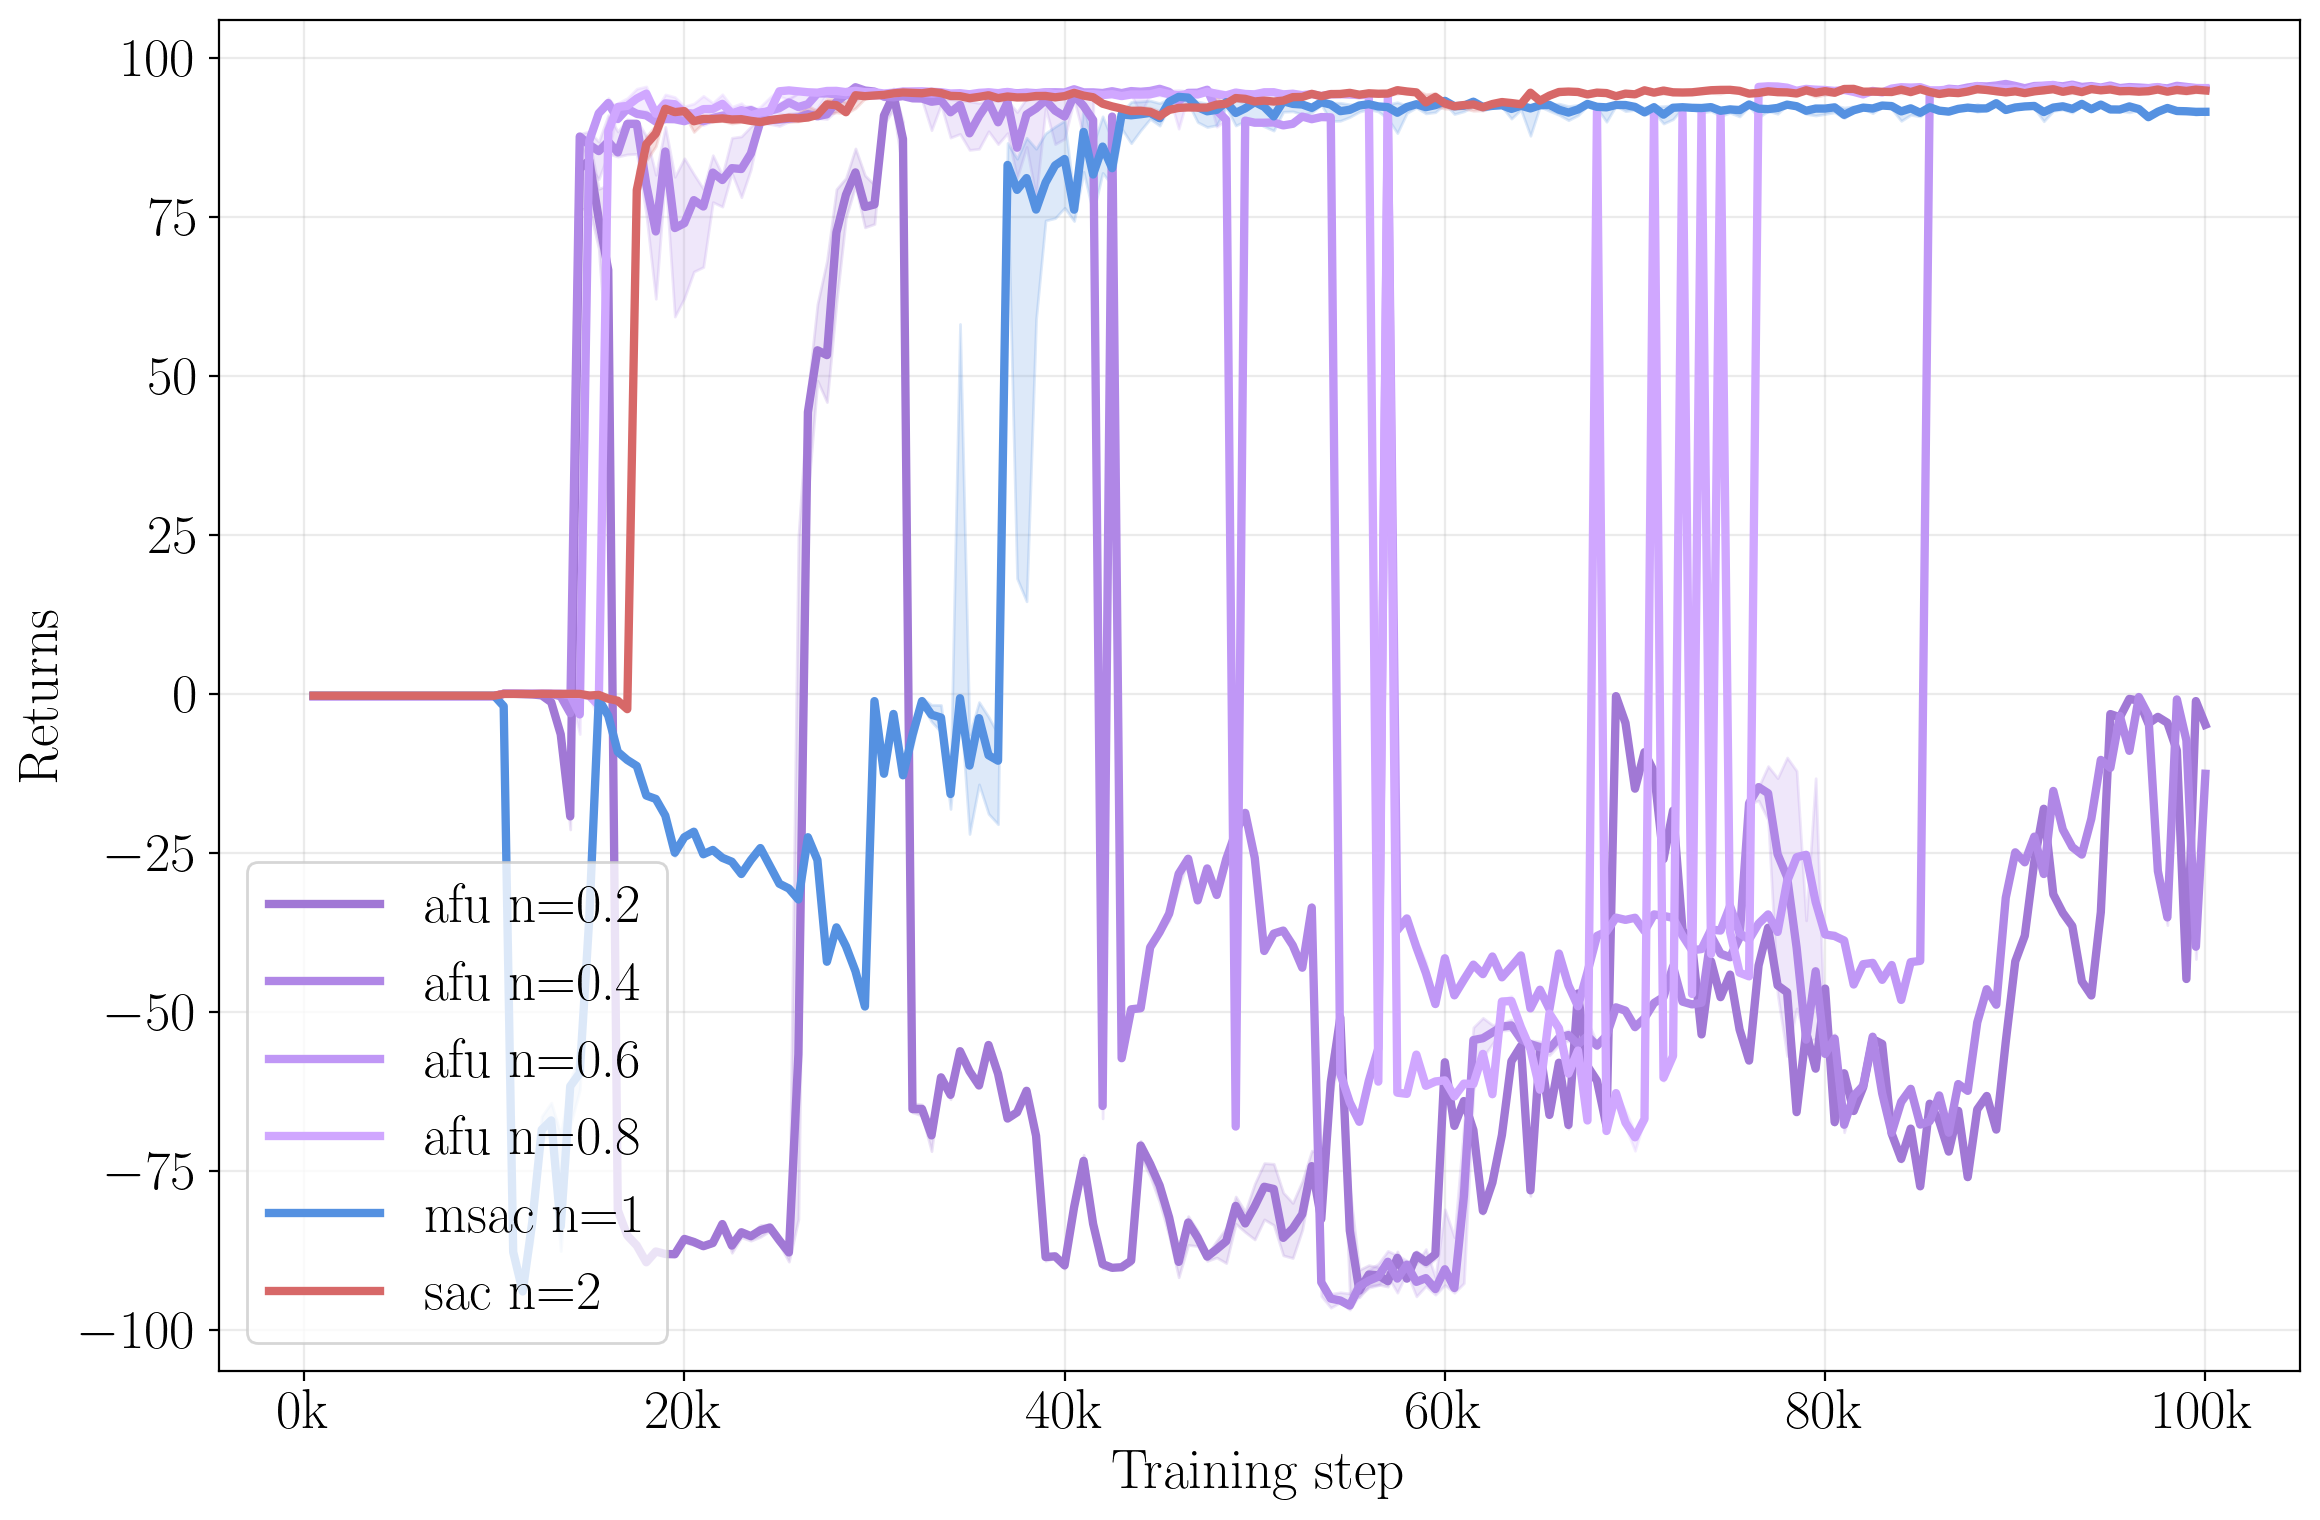
\includegraphics[width=0.3\textwidth]{../figures/env_returns_afu.png}

        \vspace{0.5cm}
        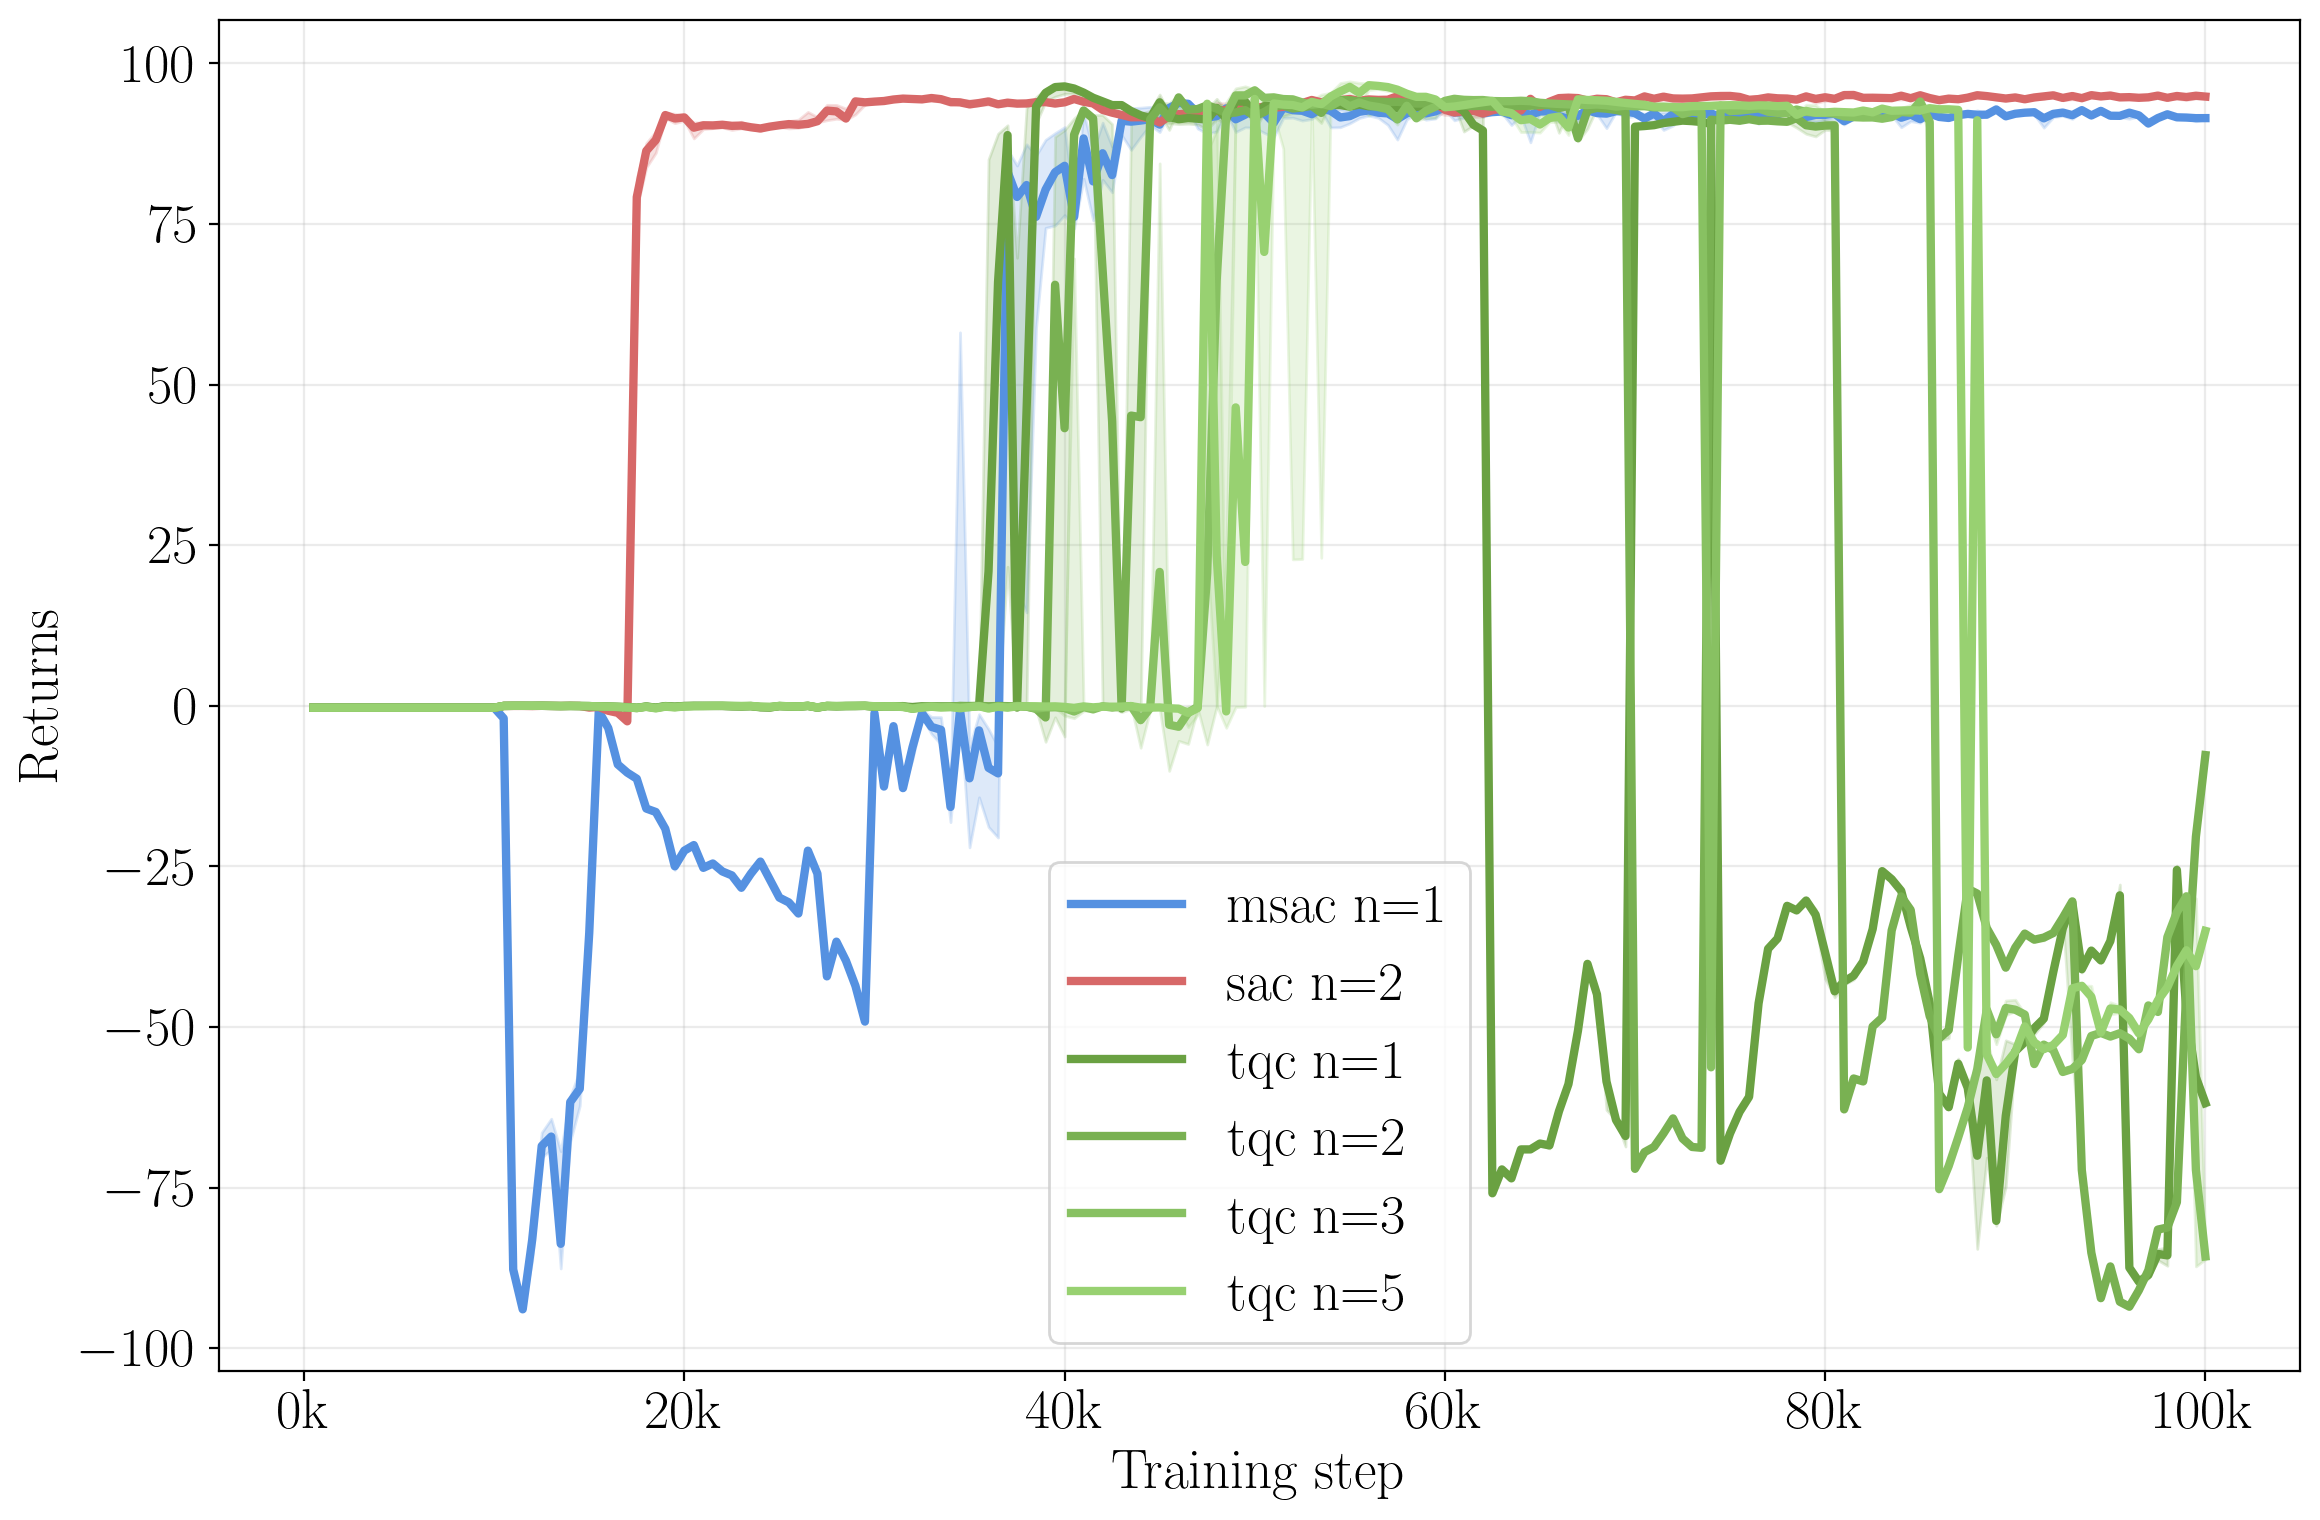
\includegraphics[width=0.3\textwidth]{../figures/env_returns_tqc.png}
        \quad
        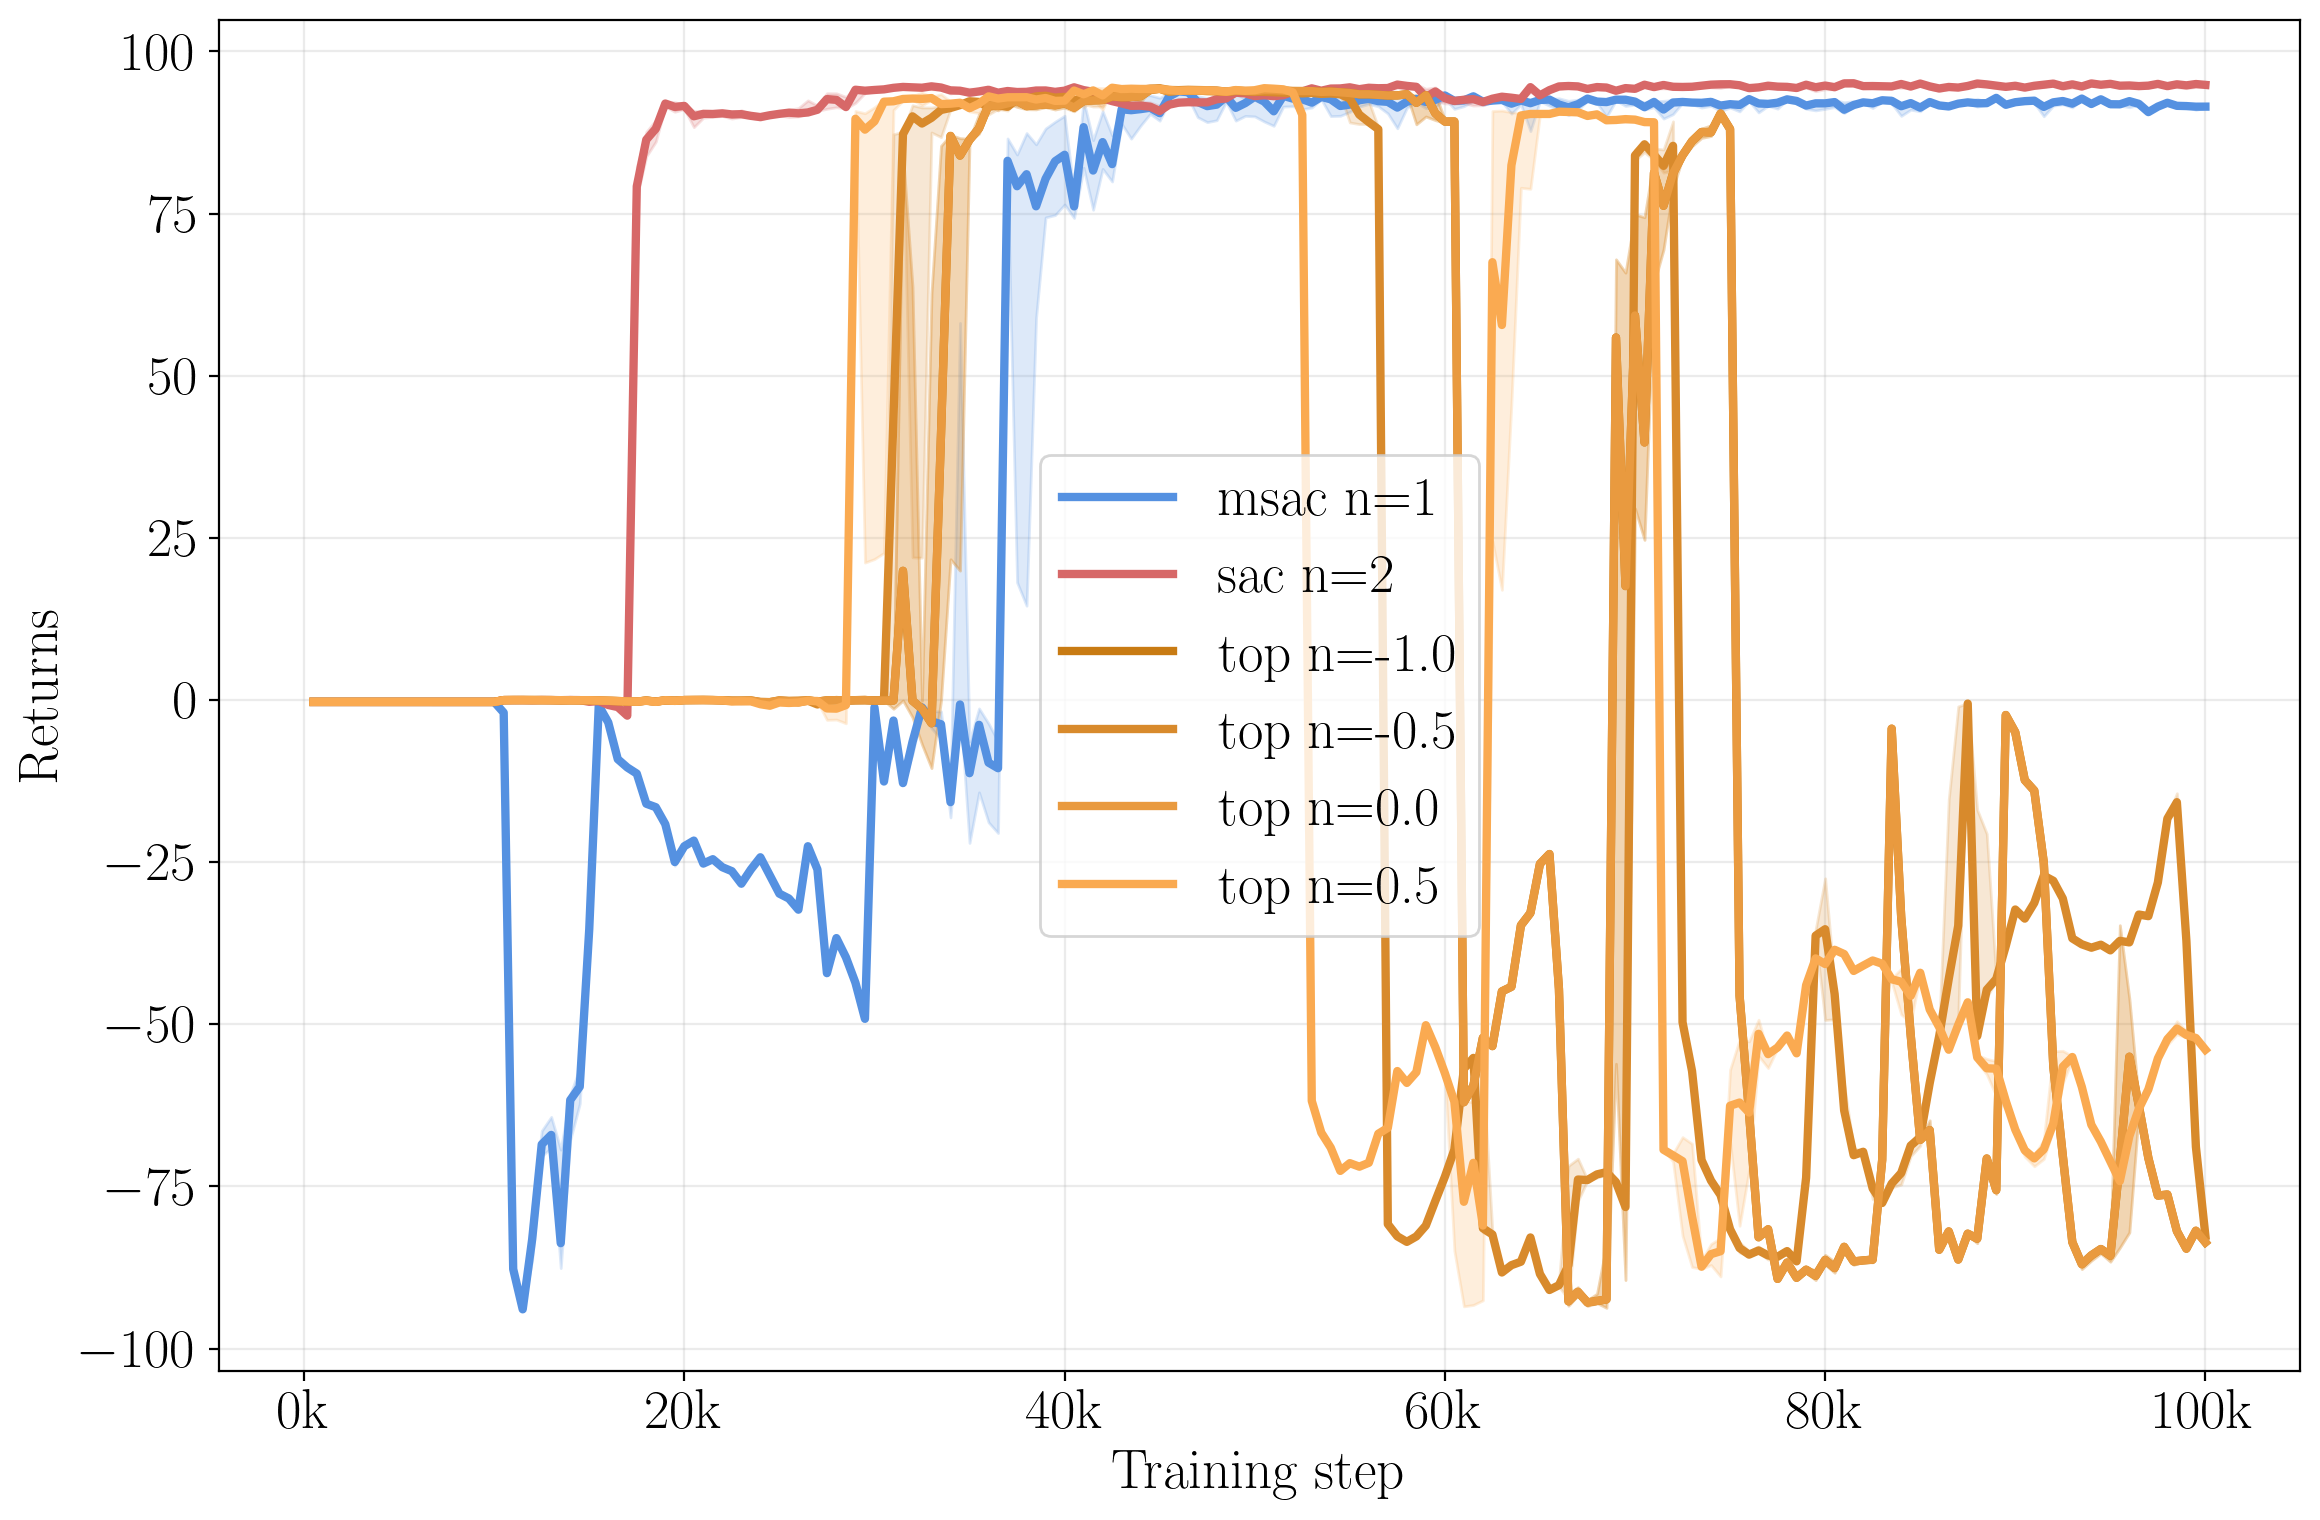
\includegraphics[width=0.3\textwidth]{../figures/env_returns_top.png}
        \caption{Évolution de la performance en fonction du temps pour chacune
        des approches. Le graphe est clair pour les approches « simples » type
        MSAC ou SAC et devient difficilement lisible pour les approches
        « complexes ». Dans l'ordre : MSAC, SAC, AFU, TQC, TOP.}
        \label{fig:performance-evolution}
    \end{figure}

    Cette absence de corrélation claire remet en question le paradigme dominant
    selon lequel on a « biais absent = bon apprentissage ». Les résultats
    suggèrent que d'autres facteurs peuvent dominer l'impact du biais sur la
    performance finale.

    Cette observation appelle une réévaluation critique des objectifs des
    méthodes de correction du biais. Si le contrôle précis du biais ne se
    traduit pas par des améliorations de performance proportionnelles, il
    devient nécessaire d'identifier les conditions où la correction du biais
    apporte des bénéfices pratiques mesurables.

    L'ensemble de ces résultats révèle la complexité sous-jacente du problème
    du biais en apprentissage par renforcement et suggère que les solutions
    proposées dans la littérature pourraient ne pas capturer entièrement les
    mécanismes en jeu.

    \section{Questions de recherche identifiées}

    Les observations empiriques révèlent la nécessité de distinguer deux types
    fondamentaux d'erreurs d'estimation qui affectent différemment
    l'apprentissage par renforcement.

    Soit $Q_\theta(s,a)$ l'estimation neuronale et $Q^\pi(s,a)$ la valeur
    vraie. Un biais uniforme s'exprime comme :

    $$
    Q_\theta(s,a) = Q^\pi(s,a) + \epsilon(s),
    $$

    où $\epsilon(s)$ est une constante pour tous les $a$ avec $s$ fixé.

    Un biais de forme préserve la valeur maximale mais altère l'ordre des
    préférences :

  $$\max_a Q_\theta(s,a) = \max_a Q^\pi(s,a) \text{ mais } \arg\max_a Q_\theta(s,a) \neq \arg\max_a Q^\pi(s,a).$$


    Le biais uniforme préserve la politique optimale car $\arg\max_a
    [Q^\pi(s,a) + \epsilon(s)] = \arg\max_a Q^\pi(s,a)$, mais se propage à
    travers le bootstrap : $Q_{t+1}(s,a) = r + \gamma[\max_{a'} Q^\pi(s',a') +
    \epsilon(s')]$. Le biais de forme brise immédiatement l'apprentissage de
    politique mais ne perturbe pas les cibles de bootstrap.

    \subsection{AFU et biais de maximisation}

    AFU présente un comportement empirique distinctif qui suggère des
    mécanismes fondamentalement différents de gestion du biais par rapport aux
    architectures acteur-critique standards.

    Comme AFU utilise directement $V(s)$ sans avoir recours à un $\arg\max$, ou
    à une opération similaire à un $\arg\max$, comme la maximisation par un
    gradient de la fonction $Q$ dans la loss de l'acteur, il n'est pas clair
    qu'AFU subisse le biais de maximisation.

    Dans AFU, les cibles de bootstrap utilisent $V(s')$ plutôt
    que $\max_{a'} Q(s',a')$. Si $V$ apprend une estimation de
    $\mathbb{E}[\max_{a'} Q(s',a')]$, cela évite le mécanisme direct de
    sélection du maximum sur des estimations bruitées qui génère le biais de
    maximisation dans les méthodes classiques.

    Le paramètre $\rho$ d'AFU influence le niveau de pessimisme de manière
    uniforme sur l'espace d'action, contrairement aux corrections par ensemble
    (TD3, SAC) où l'impact varie selon l'action sélectionnée par $\arg\max$.
    Cette uniformité pourrait expliquer la plage de contrôle du biais plus
    étendue observée empiriquement pour AFU.

    \subsection{Corrélation biais-performance}

    L'absence de corrélation claire entre contrôle du biais et performance sur
    MountainCar Continuous remet en question le paradigme dominant en
    apprentissage par renforcement continu.

    Comme montré dans le blog post, malgré des niveaux de biais variant
    largement sur une plage de valeurs Q de petite taille, tous les algorithmes
    atteignent des performances quasi-optimales. Cette observation contredit
    l'intuition selon laquelle « moins de biais = meilleur apprentissage ». Sur
    MountainCar Continuous, malgré des évolutions du biais très différentes, les
    approches qui ont un biais très faible ne semblent pas obtenir des résultats
    meilleurs que des approches simples comme SAC avec $N=2$.

    Ces observations mènent à l'étude suivante : étudier la corrélation entre
    biais et performances sur de multiples environnements pour observer s'il y
    a ou non corrélation. En plus de cela, s'il est possible de corriger le
    biais de maximisation pour isoler un biais résidu, existe-t-il une
    corrélation entre ce biais résidu et la performance ? Cela permettrait de
    mieux comprendre si l'objectif des méthodes pessimistes est
    de simplement corriger le biais de maximisation ou s'il existe un second
    objectif qui lie de l'optimisme ou du pessimisme à différentes phases de
    l'entraînement ou dans différentes régions de l'espace d'état à une
    meilleure performance.

    \subsection{Critique biaisé ou exploration}

    La focalisation exclusive sur la correction du biais au niveau des
    critiques pourrait négliger des approches alternatives plus efficaces.

    Les méthodes actuelles (TD3, TQC, TOP) appliquent le pessimisme aux
    fonctions valeur, mais cette localisation est-elle optimale ? Une
    alternative consisterait à introduire le biais directement dans
    l'apprentissage de la politique, ce qui se rapproche des mécanismes
    d'exploration.

    Il serait intéressant d'étudier quelle approche fonctionne le mieux et pourquoi :
    
    \begin{itemize}
      \item obtenir un critique parfaitement non biaisé et appliquer toutes les méthodes d'exploration au niveau de l'apprentissage de la politique ;
      \item obtenir un critique qui corrige uniquement le biais de maximisation et appliquer en plus de cela les méthodes d'exploration au niveau de l'apprentissage de la politique ;
      \item ne pas chercher à corriger le biais de maximisation et lier directement le niveau de biais au retour de l'environnement, comme ce que font des approches comme TOP.
    \end{itemize}

    Ces questions suggèrent qu'une piste de recherche pourrait être dirigée vers
    la compréhension des conditions où le biais nuit à l'apprentissage, plutôt
    que vers le développement de méthodes sophistiquées de contrôle du biais.

    \chapter{Conclusion}

    Ce stage m'a permis d'explorer quelques aspects du biais d'estimation en
    apprentissage par renforcement continu à travers l'étude de l'environnement
    MountainCar Continuous et du problème jouet de la Figure 4 de l'article
    TQC.

    L'implémentation de plusieurs algorithmes (SAC, TD3, TQC, TOP, AFU) dans un
    cadre uniforme a facilité leur comparaison et permis de reproduire
    certaines expériences de la littérature. Cette approche a révélé une erreur
    méthodologique dans la reproduction de la Figure 4 de l'article TQC :
    l'absence de réseaux cibles créait des instabilités qui masquaient les
    véritables comportements des algorithmes.
    
    L'étude d'AFU suggère des comportements potentiellement différents des
    autres méthodes acteur-critique, notamment dans la gestion du biais via le
    paramètre $\rho$. Cependant, ces observations restent préliminaires et
    nécessiteraient une validation sur davantage d'environnements pour être
    confirmées.

    Sur MountainCar Continuous, les résultats ne montrent pas de corrélation
    claire entre niveau de biais et performance d'apprentissage, ce qui soulève
    des questions sur l'importance pratique de la correction du biais dans
    certains contextes.

    Ce travail comporte des limites : l'analyse se concentre sur un seul
    environnement relativement simple, les contraintes computationnelles ont
    restreint l'étendue des évaluations et les difficultés associées à AFU-TQC
    illustre la complexité d'hybridation entre architectures différentes.

    Ces observations soulèvent des questions sur les conditions où la
    correction du biais apporte réellement des bénéfices pratiques et sur les
    mécanismes sous-jacents de propagation du biais. Une extension de cette
    étude à des environnements plus variés serait nécessaire pour valider ou
    infirmer ces premières observations.

    Je tiens à remercier M. Olivier Sigaud pour son encadrement, ses conseils
    et le temps qu'il a consacré à ce stage.
    
    \printbibliography

\end{document}
